\documentclass[pdflatex,sn-mathphys-num]{sn-jnl}% Math and Physical Sciences Numbered
\usepackage{comment}

\usepackage{graphicx}
\usepackage{tabularx,booktabs}
\usepackage{amsmath}
\usepackage{xcolor}
\usepackage{enumitem}
\usepackage{fancyhdr}
\usepackage{caption}
\usepackage{textcomp}
\usepackage{listings}
\usepackage{tikz}
\newcommand{\logref}[1]{\textit{(Log File, #1)}}

\usetikzlibrary{positioning,arrows.meta}

\pagestyle{fancy}
\fancyhf{}
\lhead{\small Proyecto IK-Dron}
\rhead{\small Log File}
\cfoot{\thepage}
\setlength{\headheight}{14pt}

\begin{document}

%% ============================== PORTADA ==============================
\begin{titlepage}
\centering
{\large Universidad Autónoma de Aguascalientes\par}
{\normalsize Departamento de Sistemas Electrónicos\par}
\vspace{3.5cm}
{\Huge\bfseries IK-Dron\par}
\vspace{0.5cm}
{\Large Desarrollo y puesta en vuelo de un dron de carreras\\ de 5 pulgadas con BetaFlight\par}
\vspace{0.8cm}
{\large LogFile (Bitácora Técnica)\par}
\vspace{3cm}
{\large Contreras R. Orlando\\ Garcia B. Iker\par}
\vspace{1cm}
{\normalsize \textbf{Asesor:} Dr. Luis Antonio Raygoza Pérez\par}
\vfill
{\normalsize Aguascalientes, Ags., octubre de 2026\par}
\end{titlepage}
%%==================================%%
%% Sample for unstructured abstract %%
%%==================================%%


%%==================================%%
%% Sample for structured abstract %%
%%==================================%%



%%\pacs[JEL Classification]{D8, H51}

%%\pacs[MSC Classification]{35A01, 65L10, 65L12, 65L20, 65L70}

\newpage

\begin{figure}[!h]
    \centering
    
\includegraphics[width=0.8\linewidth]{src/QR.png}
    \label{fig:placeholder}
\end{figure}
\tableofcontents
\newpage

\section{Marzo 2026}
\subsection{Marzo 13 \label{sec:3-13}}
\subsubsection{Aprendizajes}
Primeras pruebas de vuelo, recibimos el dron tal y como se ve en la figura
\ref{fig:Dron1}, el cual es un dron de carreras, con una estructura de fibra de carbono, motores brushless, controladora de vuelo, ESCs y una batería LiPo. El dron se encuentra en buenas condiciones, sin embargo.
Se recibieron instrucciones de como utilizarlo por el docente Luis Antonio Raygoza Perez resltando los siguientes puntos
\begin{itemize}
    \item Antes de energizar el dron se debe de setear el control en las perillas por default tal y como se ve en la imagen \ref{fig:Control}, esto es para evitar que el dron se mueva de forma inesperada al energizarlo.
    \item Al momento de energizar el dron, se debe de conectar con una mano y con la otra mano se debe de mantener el dron en el suelo, esto es para evitar que el dron se eleve de forma inesperada al energizarlo.
    \item Al momento de cargarlo, se debe revisar cada celda esto se hace con un checador de baterías, conectando negativo con negativo para evitar hacer corto como se aprecia en la figura \ref{fig:Medidor}
\end{itemize}


\begin{figure}[!h]
    \centering
    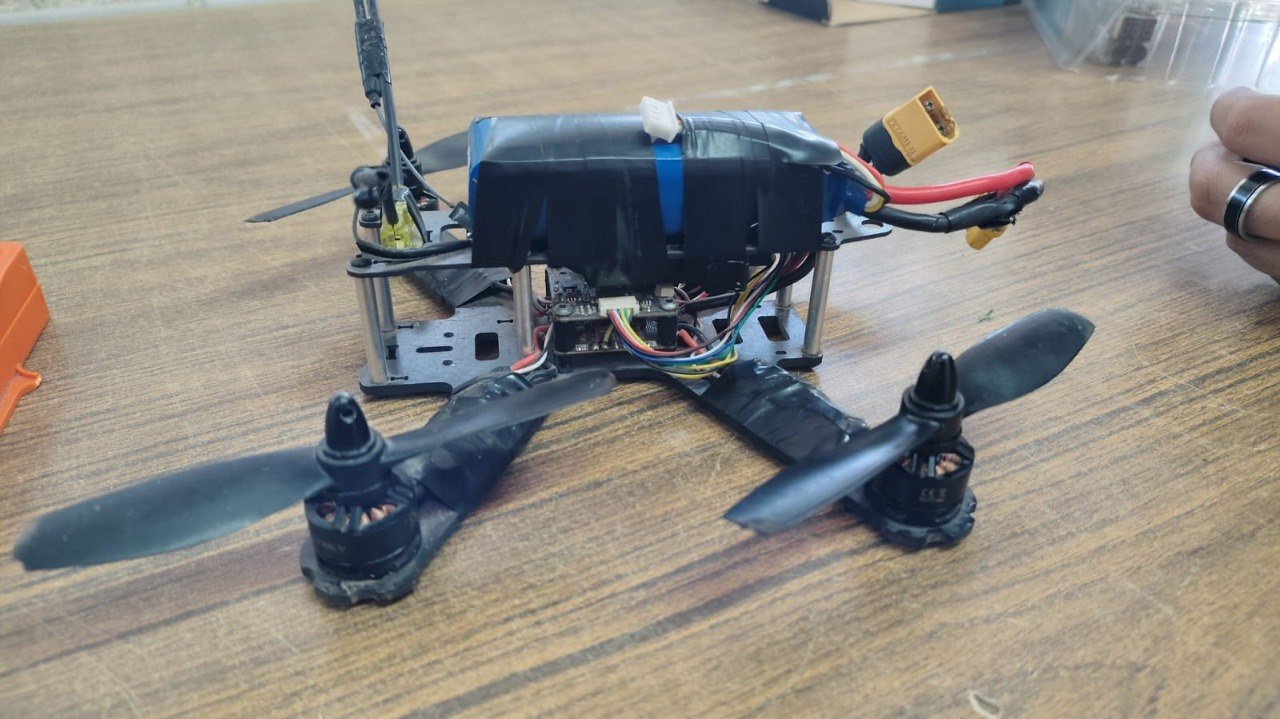
\includegraphics[width=0.5\linewidth]{src//srclog/3-13Dron.png}
    \caption{Dron recibido [Marzo 13, 2026]}
    \label{fig:Dron1}
\end{figure}

\begin{figure}[!h]
    \centering
    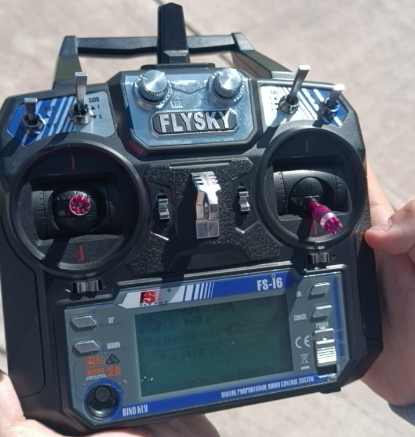
\includegraphics[width=0.5\linewidth]{src//srclog/Control.png}
    \caption{Control con perillas en default}
    \label{fig:Control}
\end{figure}

\begin{figure}
    \centering
    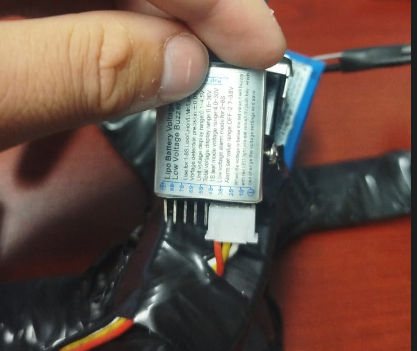
\includegraphics[width=0.5\linewidth]{src/srclog/Checador.png}
    \caption{Checador de baterías}
    \label{fig:Medidor}
\end{figure}
\subsubsection{Incidentes y puntos de mejora}
Al realizar las pruebas de vuelo, ocurrieron dos incidentes
\begin{itemize}
    \item Una de las tuercas que sujeccionan las helices no estaba bien apretada por lo que salió volando, fue aqui donde empezamos a tomar nota de todo lo que teníamos para el caso de refacciones.
    \item El cable de la batería no estaba bien sujetado y hubo un momento donde la helice lo cortó por lo que actuamos con cuidado y paramos la operación.
\end{itemize}
Frente a estos dos incidentes, se tomaron las siguientes medidas
Realizar una tabla de componentes y refacciones, esto es para tener un control de lo que tenemos y lo que necesitamos, así como para tener un control de los costos, esta tabla se muestra en el anexo \ref{sec:TablaComponentes}.
Mientras que para el cable de la batería fue una oportunidad debido a que debíamos incorporar un switch para no estar conectando y desconectando la batería, por lo que se decidió incorporar un switch para evitar este tipo de incidentes en el futuro, esto se hizo con un switch de 1 polos y 2 posiciones. Este switch fue incorporado hasta la sección \ref{sec:4-1}

Además el lugar nos pareció un poco pequeño para realizar las pruebas de vuelo, por lo que se decidió buscar un lugar más amplio para realizar las pruebas, además de que fuera un lugar donde sea facil localizar componentes en caso de desprendimiento, esto se logró en la sección \ref{sec:3-27}.

\subsection{27 Marzo \label{sec:3-27}}
\subsubsection{Aprendizajes}
Nos empezamos a familiarizar con el software de librePilot, guardamos la configuración del dron, y empezamos a realizar configuraciones. Al realizar las configuraciones nos dimos cuenta de varios puntos
\begin{itemize}
\item Las configuraciones se deben de realizar con el dron \textbf{desarmado} es decir con la configuración en desarmado tal y como se muestra en la figura \ref{fig:lpArmed},
\item Para que se guarde la configuración se debe conectar con la batería y cargar el dron, esto es algo que no se había hecho antes, por lo que se habían perdido las configuraciones realizadas.
\item Para actualizar el firmware se debe ejecutar la secuencia anexada en \ref{sec:Firmware}
\item Para configurar el control se debe de realizar con el dron desarmado, para esto nosotros nos basamos en el video \cite{TorrenteDigital}, la configuración previa realizada por la primera generación se detalla en el documento de Desarrollo

\end{itemize}

\begin{figure}[!h]
    \centering
    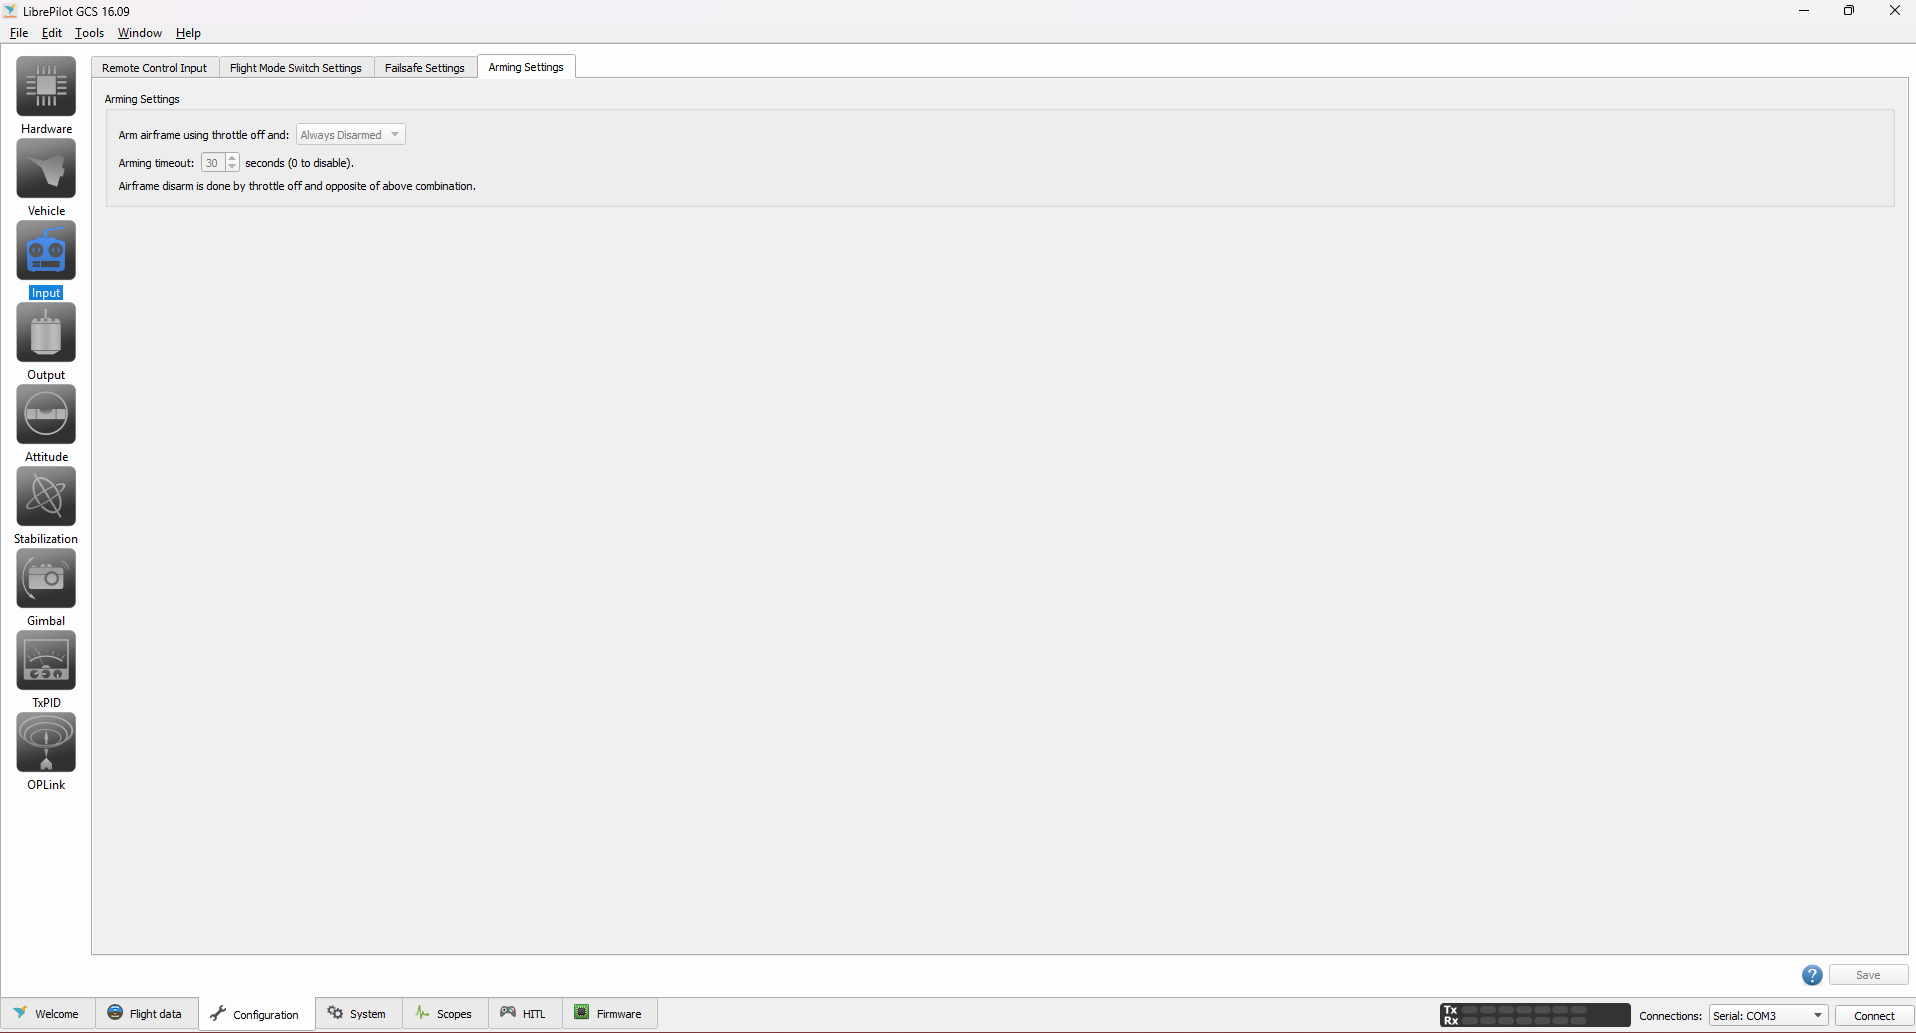
\includegraphics[width=\linewidth]{src//srclog/Disarmed.png}
    \caption{Dron en estado desarmado}
    \label{fig:lpArmed}
\end{figure}

Realizamos una configuración personalizada para mejorar la respuesta del control, ajustando los parámetros de \textit{CruiseControl} y modificando la curva del acelerador (\textit{throttle}).

\subsubsection{Incidentes y puntos de mejora}
Este día obtuvimos autorización para realizar pruebas en el estadio de la institución, un espacio más seguro y amplio. Logramos un mejor control del vuelo, aunque notamos que el dron tendía a inclinarse hacia un lado, como se aprecia en la imagen \ref{fig:lado}.

\begin{figure}[!h]
    \centering
    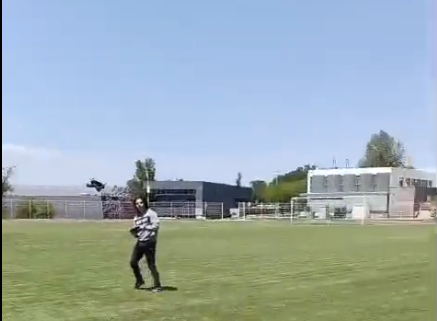
\includegraphics[width=0.5\linewidth]{src//srclog/lado.png}
    \caption{Dron inclinado hacia un lado durante el vuelo}
    \label{fig:lado}
\end{figure}

Respecto a los incidentes presentados:
\begin{itemize}
    \item Personal de seguridad se acercó para verificar que el equipo no contara con cámara y nos advirtió sobre las restricciones de altura sin permisos especiales, sugiriéndonos evitar zonas cercanas a aulas y vehículos. Aprovechamos para consultar sobre áreas permitidas y nos validaron el uso del estadio sin requerir trámites adicionales.
    \item Durante las pruebas en el estadio, el dron sufrió una caída que fracturó una de las antenas del controlador de vuelo, generando un falso contacto intermitente que obligó a programar su reparación.
\end{itemize}
\newpage

\section{Abril 2026}
\subsection{1 de Abril \label{sec:4-1}}
\subsubsection{Aprendizajes}
Esta jornada se destinó a resolver los incidentes reportados en la sección \ref{sec:3-27}. Se reparó la antena del controlador de vuelo y se instaló físicamente el interruptor de encendido para evitar el riesgo detectado en la sección \ref{sec:3-13}. El resultado se observa en la figura \ref{fig:Reparacion}.

\begin{figure}[!h]
    \centering
    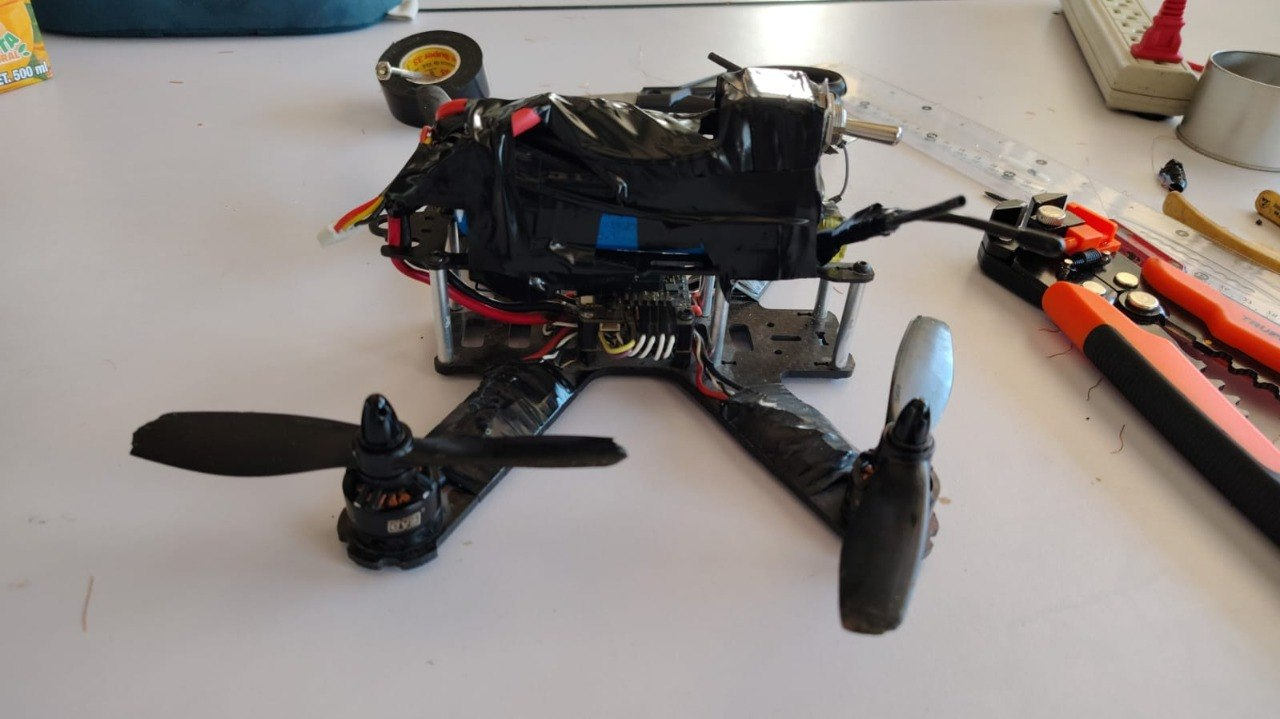
\includegraphics[width=0.5\linewidth]{src//srclog/4-1Reparacion.png}
    \caption{Reparación de antena e integración del interruptor de encendido}
    \label{fig:Reparacion}
\end{figure}

\subsubsection{Incidentes y puntos de mejora}
Durante la soldadura del interruptor, se generó un puente de continuidad accidental con la línea de la batería, provocando un chispazo sin mayores afectaciones. Como punto de mejora, se evaluó reemplazar la cinta de aislar utilizada para sujetar la batería por un arnés de velcro o una banda elástica, facilitando su extracción y garantizando mayor firmeza.

\subsection{10 de Abril \label{sec:4-10}}
\subsubsection{Aprendizajes}
Se intentó realizar una sesión de pruebas de vuelo, pero surgió un problema de comunicación entre el dron y la computadora: aunque el sistema reconocía el puerto, no permitía cargar configuraciones. Se intentó actualizar el firmware sin éxito (el software identificaba la conexión pero bloqueaba la escritura, como se muestra en la figura \ref{fig:Firmwarefalla}). Como último recurso, se intentó establecer comunicación serial directa mediante un script en Python a distintas frecuencias de baudios.

\begin{comment}
\begin{figure}[!h]
    \centering
    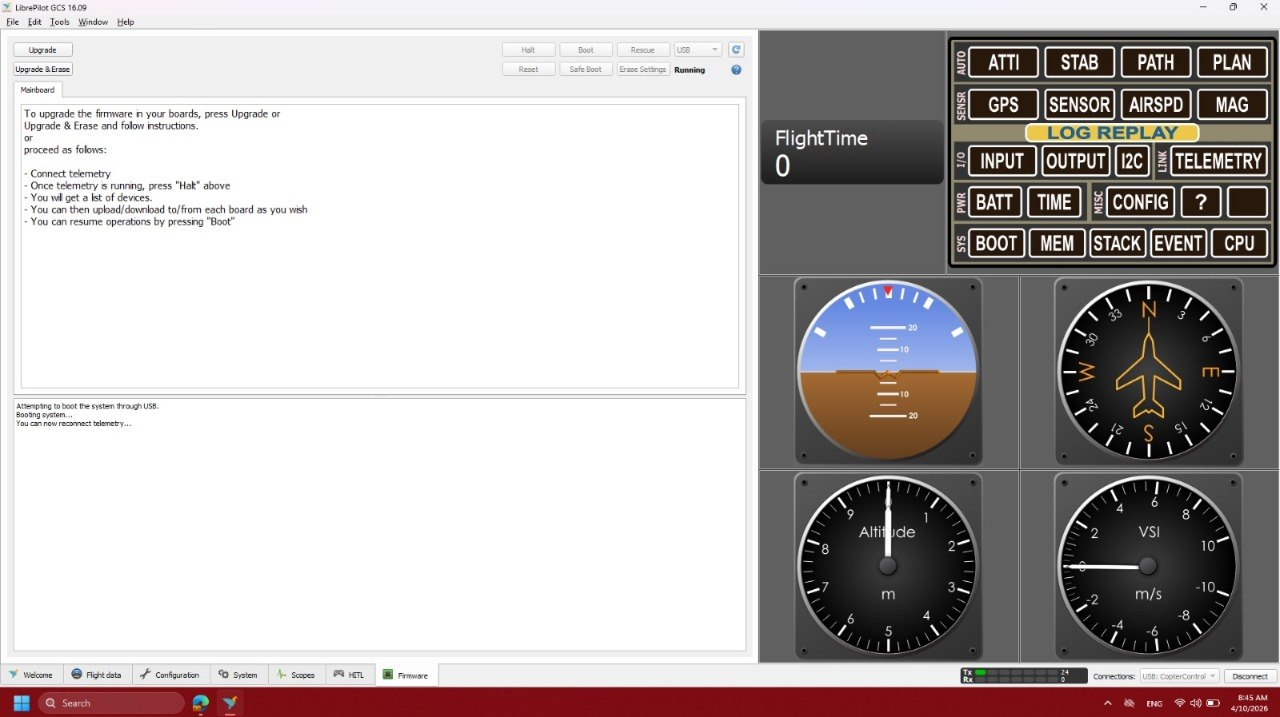
\includegraphics[width=0.8\linewidth]{src//srclog/Firmwarefalla.png}
    \caption{Falla al intentar actualizar el firmware}
    \label{fig:Firmwarefalla}
\end{figure}
\end{comment}

\subsubsection{Incidentes y puntos de mejora}
Dado que el objetivo inicial era portear el firmware a BetaFlight, este fallo en la controladora motivó la búsqueda de una tarjeta compatible con dicho entorno. Tras consultar la situación con el Dr. Raygoza, la recomendación fue intentar un restablecimiento profundo (\textit{hard reset}) o, de lo contrario, reemplazar la controladora para permitir configuraciones avanzadas.

\subsection{12 de Abril}
\subsubsection{Aprendizajes}
Se dedicó la jornada a la documentación del proyecto, recopilación de material gráfico y creación del repositorio oficial en GitHub para el control de versiones y almacenamiento de recursos.
\subsubsection{Incidentes y puntos de mejora}
No se registraron incidentes. Se identificó la falta de un registro fotográfico y en video más constante de las pruebas, por lo que se acordó mejorar esta cobertura en futuras sesiones.

\section{Mayo 2026}
\subsection{15 de Mayo}
\subsubsection{Aprendizajes}
Se diagnosticó a fondo la tarjeta del dron, identificando que el componente dañado era la placa AIO (\textit{All in One}), la cual integra el microcontrolador, los sensores y los ESCs. El circuito principal corresponde a un microcontrolador STM32F103C8T6 (visible en la figura \ref{fig:CC3D EVO}).

\begin{figure}[!h]
    \centering
    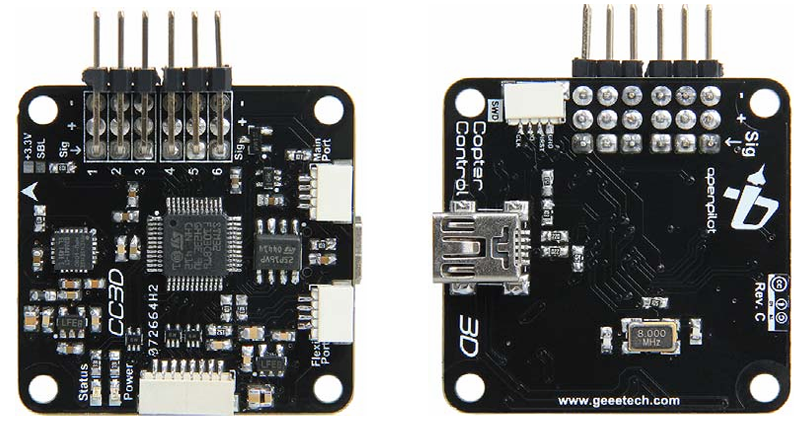
\includegraphics[width=0.8\linewidth]{src//srclog/CC3D.png}
    \caption{Controladora de vuelo CC3D EVO}
    \label{fig:CC3D EVO}
\end{figure}

Localizamos los pines de programación SWD en la parte inferior de la placa mediante el rastreo de pistas físicas (figura \ref{fig:SWDConector}), con el propósito de intentar un reseteo de fábrica por hardware.

\begin{figure}[!h]
    \centering
    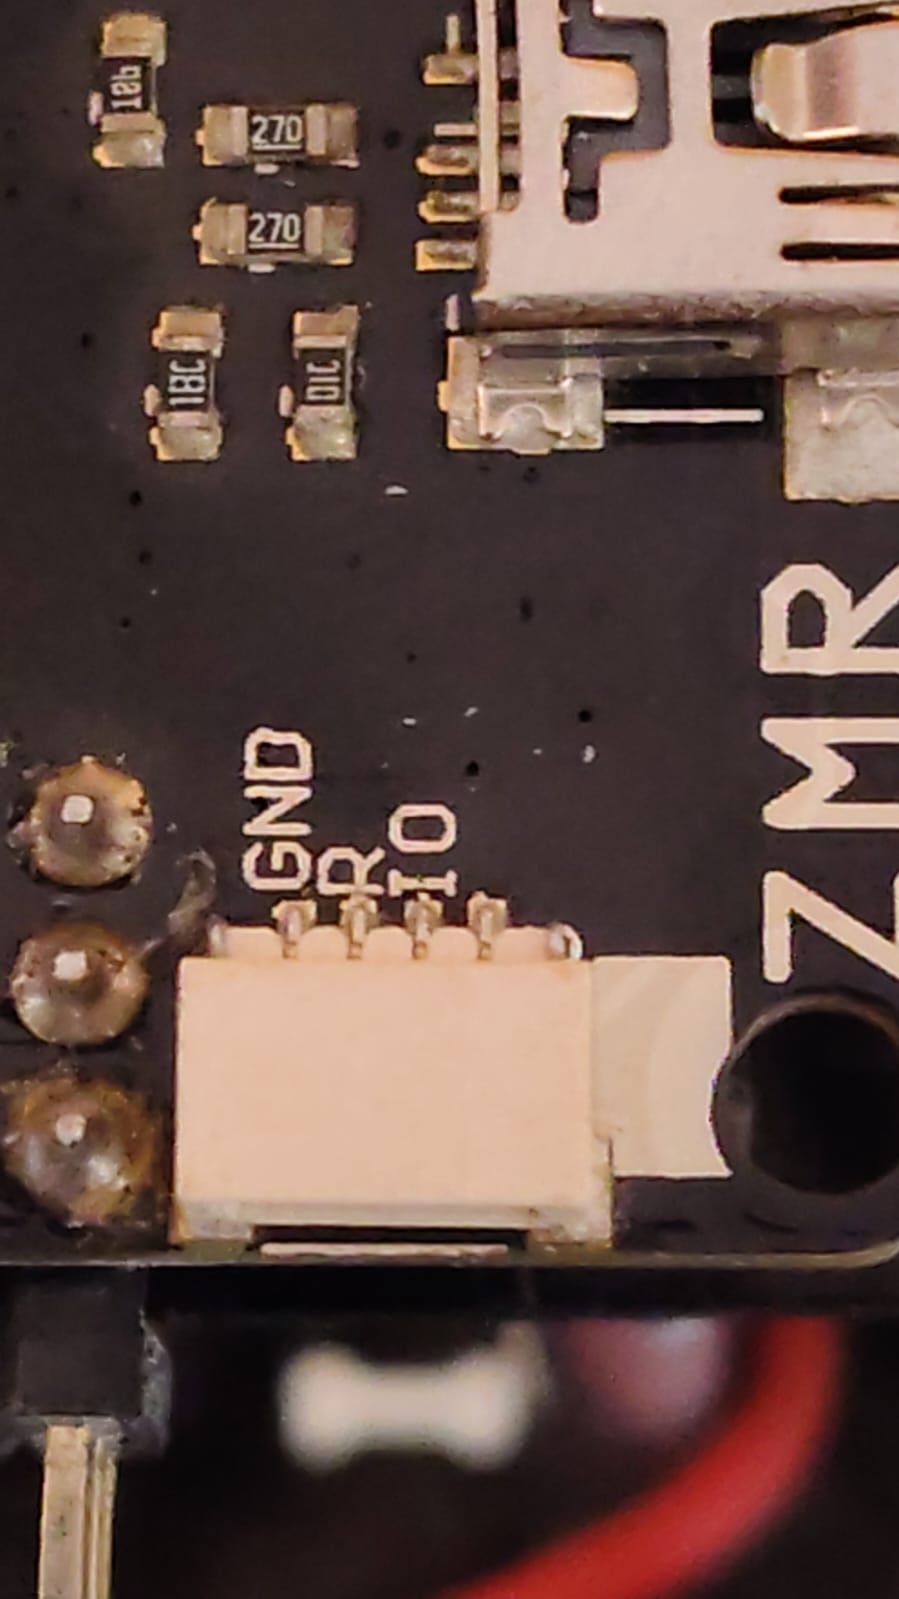
\includegraphics[width=0.5\linewidth, angle=270]{src//srclog/SWD.png}
    \caption{Conector SWD localizado en la placa}
    \label{fig:SWDConector}
\end{figure}



\subsection{27 de Mayo \label{sec:5-27}}
\subsubsection{Aprendizajes}
Nos costó trabajo conseguir el conector del SWD, estuvimos intentando con diferentes, sin embargo no logramos encontrarlo, por lo que nos quedaban dos opciones
\begin{itemize}
    \item Pedir el conector por aliexpress, esperando que nos llegue en uno o dos meses.
    \item Soldarle Cables al cable expuesto del conector para intentar hacer la comunicación.
\end{itemize}

Finalmente nos decantamos por la segunda opción, por lo que se procedió a soldar cables al conector, para esto se identificaron los pines del conector, los cuales son VCC, GND, SWDIO y SWCLK, esto se hizo con la ayuda de un multímetro para identificar la continuidad entre los pines del conector y los pines del microcontrolador, esto se muestra en la figura \ref{fig:SWDIdentificacion}. Se debe reconocer el trabajo que hizo Iker Garcia para soldar los cables al conector, ya que fue un trabajo delicado debido a que el conector es pequeño y los pines están muy juntos, por lo que se debe tener cuidado para no hacer corto entre los pines, esto se logró gracias a la paciencia y habilidad de Iker Garcia.

\begin{figure}[!h]
    \centering
    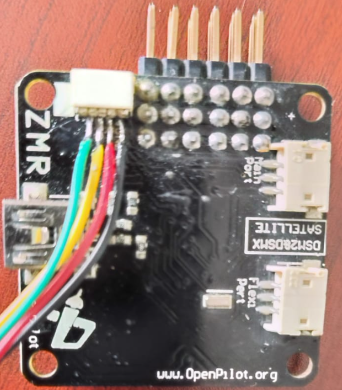
\includegraphics[width=0.5\linewidth]{src//srclog/SWDSoldados.png}
    \caption{Cables soldados al puerto SWD}
    \label{fig:SWDIdentificacion}
\end{figure}

Se procedió a hacer entonces un hard-reset con STM32CUBE Programmer, para esto se conectó el conector al programador, y se intentó hacer el hard-reset, sin embargo no se logró establecer la comunicación con el microcontrolador, por lo que se intentó con diferentes frecuencias de comunicación, así como diferentes configuraciones del programador, sin embargo no se logró establecer la comunicación, esto nos llevó a la conclusión de que el microcontrolador está dañado, por lo que se deberá de reemplazar la placa AIO para poder seguir avanzando en el proyecto.


\newpage
\section{Junio 2026}
\subsection{2 de Junio \label{sec:6-2}}
\subsubsection{Aprendizajes}
La placa CC3D se quemó, y a pesar de los intentos por recuperarla y repararla (actualización de firmware, comunicación serial y \textit{hard reset} por SWD, secciones \ref{sec:4-10} a \ref{sec:5-27}) no fue posible volver a comunicarse con el microcontrolador. Por esta razón se decidió reemplazarla por una nueva controladora de vuelo, aprovechando el cambio para migrar a BetaFlight, que era uno de los objetivos planteados desde la sección \ref{sec:4-10}. Este día se dedicó a investigar BetaFlight y las controladoras de vuelo disponibles, considerando los siguientes puntos:
\begin{itemize}
    \item La CC3D utiliza un procesador STM32F103 (72\,MHz), cuyo soporte fue retirado en las versiones recientes de BetaFlight.
    \item Las tarjetas actuales emplean procesadores F405 (168\,MHz), económicos y altamente capaces para drones de 5 pulgadas \cite{stm32ventajas}.
    \item BetaFlight ofrece una comunidad activa, modos de estabilización avanzados (Angle y Horizon) y configuración mediante interfaz gráfica o terminal (CLI).
\end{itemize}

Se seleccionó la \textbf{SpeedyBee F405 V4}, debido a:
\begin{itemize}
    \item Procesador STM32F405 compatible con la versión actual de BetaFlight.
    \item Factor de forma de 30.5\,$\times$\,30.5\,mm, compatible con el chassi LS210.
    \item Se adquiere en formato \textit{stack} junto a un ESC 4 en 1 de 55 A, simplificando drásticamente el cableado y eliminando la necesidad de una PDB independiente.
    \item Permite configuración inalámbrica por Bluetooth mediante la aplicación móvil.
\end{itemize}


\subsection{10 de junio}
\subsubsection{Aprendizajes}
Mientras se investigaba sobre otras controladoras del dron adecuadas. Se contempló la posibilidad de comprar una base de pruebas para hacer ajustes en PID en vivo. Se estuvo revisando en cuanto a precios y la mejor alternativa era fabricar una entonces se tomo una base de ventilador para el soporte y en la parte superior se adaptó.


\begin{figure}[!h]
    \centering
    % Primera figura (izquierda)
    \begin{minipage}[b]{0.48\textwidth}
    \centering
    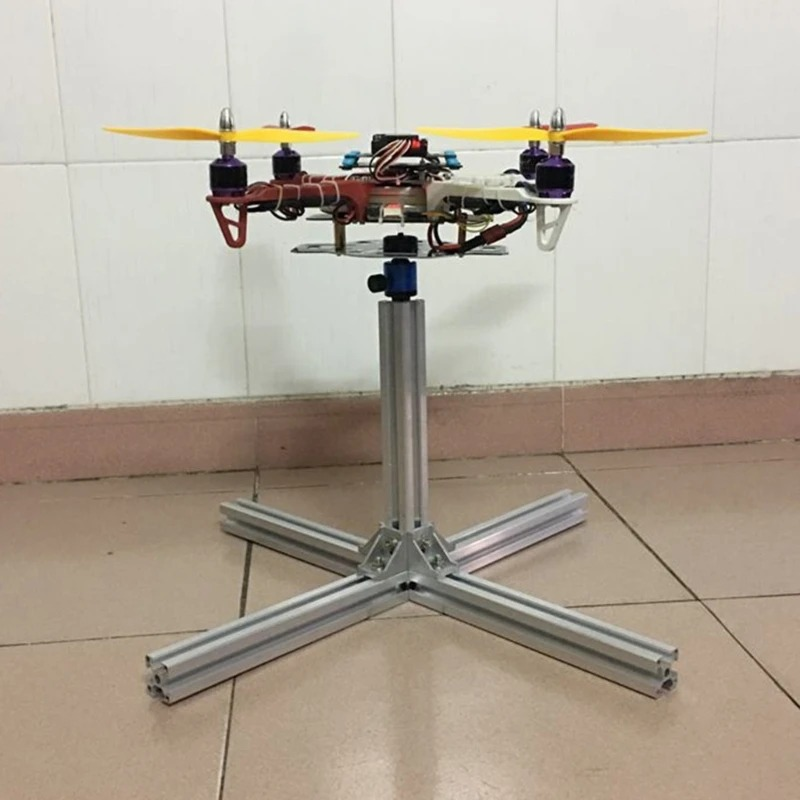
\includegraphics[width=0.8\linewidth]{src/srclog/BaseRef.png}
    \caption{Base referencia}
    \label{fig:BaseRef}
    \end{minipage}
    \hfill % Espacio horizontal entre las dos figuras
    % Segunda figura (derecha)
    \begin{minipage}[b]{0.48\textwidth}
    \centering
    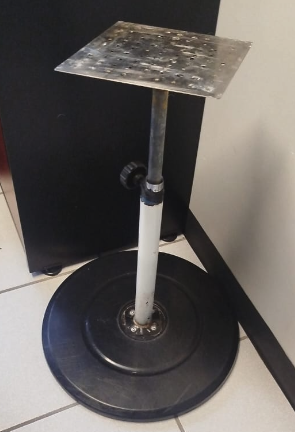
\includegraphics[width=0.5\linewidth]{src/srclog/Base.png}
    \caption{Base fabricada}
    \label{fig:Base}
    \end{minipage}
\end{figure}



\subsection{23 de junio}
\subsubsection{Aprendizajes}


Para asegurar completa compatibilidad se consideró el tamaño de la placa
La Speedybee (la nueva) mide 40 mm (4 mm mas que la CC3D evo) mientras que \textbf{la distancia entre los agujeros es la misma }entre las dos placas, la Speedybee tiene un diametro de 4 mm (1 mm mas que la CC3D evo)

En cuanto a dimensiones de la carcasa, la CC3D Evo quedaba justo (mide 36 mm, anexo imagen), entonces quedaria un poco salida de ambos lados. y en cuanto a la altura mide 35 mm esta sobrado en cuanto a alturar porque las dos placas de la Speedy Bee suman 15 mm como altura ya de ahi seria considerar las separaciones

\begin{figure}[htbp]
    \centering
    % Primera figura (izquierda)
    \begin{minipage}[b]{0.48\textwidth}
        \centering
        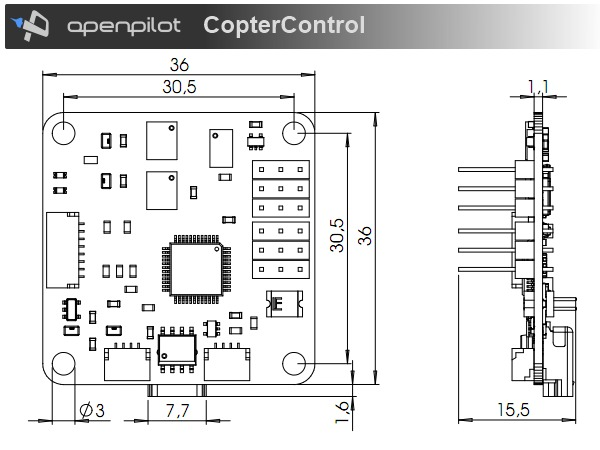
\includegraphics[width=\linewidth]{src/srclog/Medidas Copter CC3D.png}
        \caption{Medidas CC3D Evo}
        \label{fig:cc3d}
    \end{minipage}
    \hfill % Espacio horizontal entre las dos figuras
    % Segunda figura (derecha)
    \begin{minipage}[b]{0.48\textwidth}
        \centering
        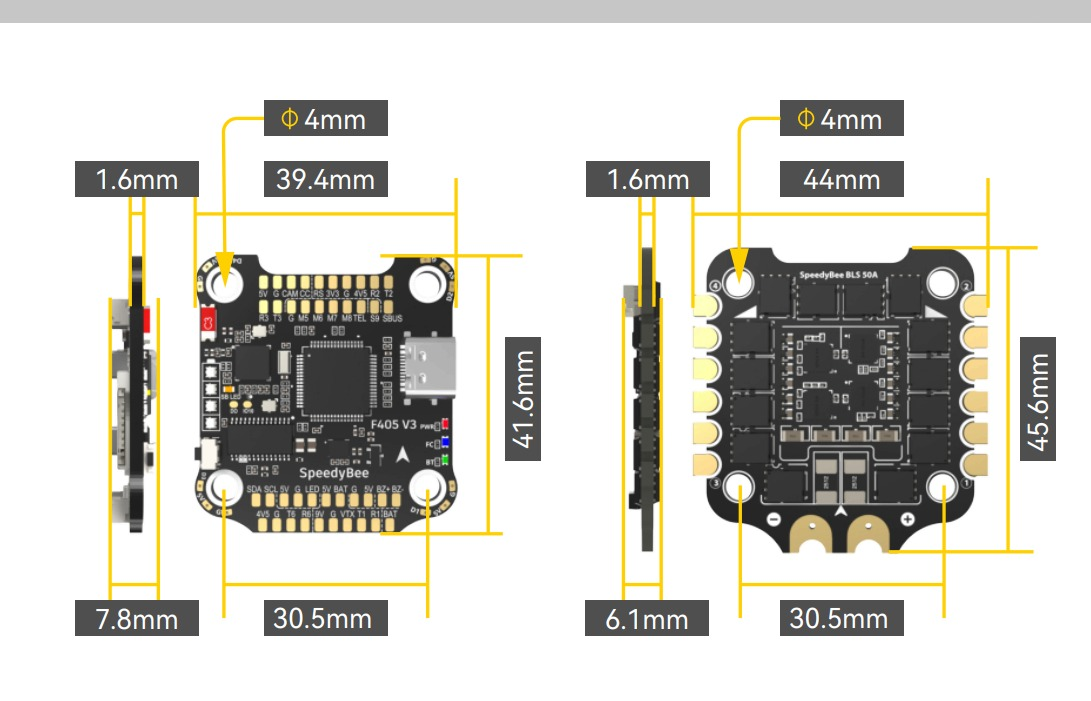
\includegraphics[width=1.1\linewidth]{src/srclog/SPidibitamano.png}
        \caption{Medidas SpeedyBee v4}
        \label{fig:speedybee}
    \end{minipage}
\end{figure}



\begin{figure}[!h]
    \centering
    % Primera figura (izquierda)
    \begin{minipage}[b]{0.48\textwidth}
    \centering
    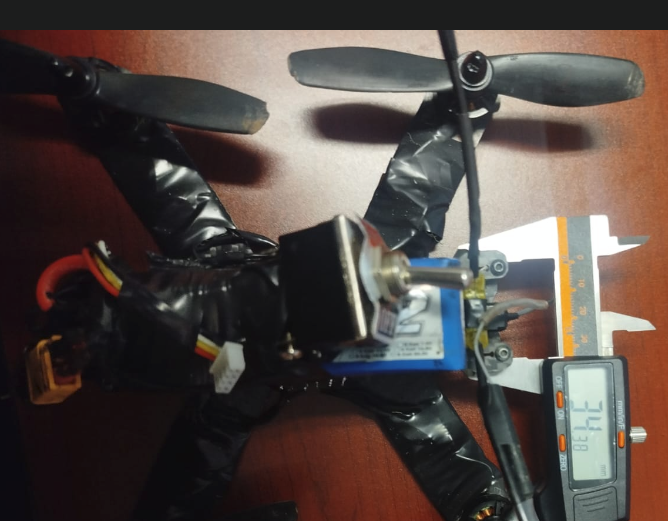
\includegraphics[width=\linewidth, angle =90]{src/srclog/Anchura.png}
    \caption{Medición Anchura Frame LS-210}
    \label{fig:Anchura}
    \end{minipage}
    \hfill % Espacio horizontal entre las dos figuras
    % Segunda figura (derecha)
    \begin{minipage}[b]{0.48\textwidth}
    \centering
    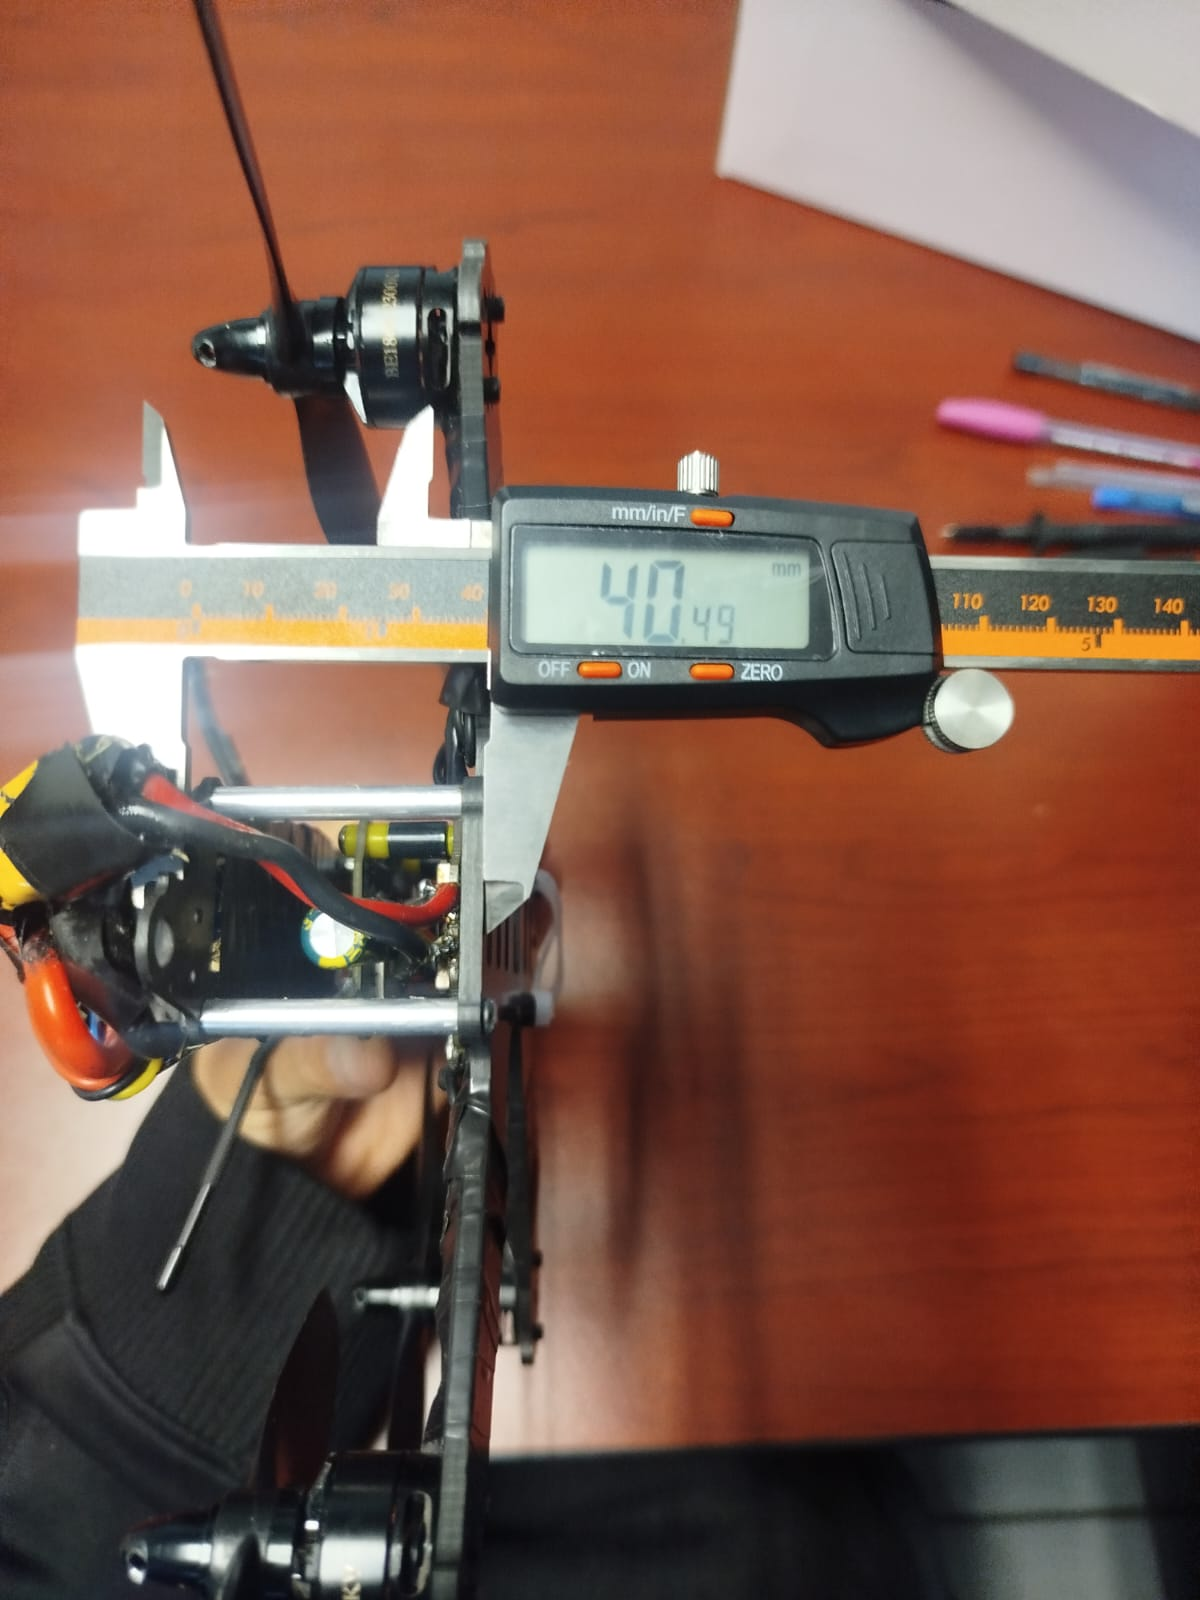
\includegraphics[width=0.8\linewidth]{src/srclog/Altura.png}
    \caption{Medición Altura Frame LS-210}
    \label{fig:Altura}
    \end{minipage}
\end{figure}



\section{Agosto 2026}
\subsection{28 de Agosto \label{sec:8-28}}
\subsubsection{Aprendizajes}
Se retiró la vieja CC3D y se instaló el nuevo \textit{stack} SpeedyBee F405 V4. Se conectó la tarjeta al configurador de BetaFlight y se actualizó el firmware a la versión 4.4.3 utilizando el \textit{target} \texttt{SPEEDYBEEF405V4} (figuras \ref{fig:8-28Config} y \ref{fig:8-28Updated}).

\begin{figure}[!h]
    \centering
    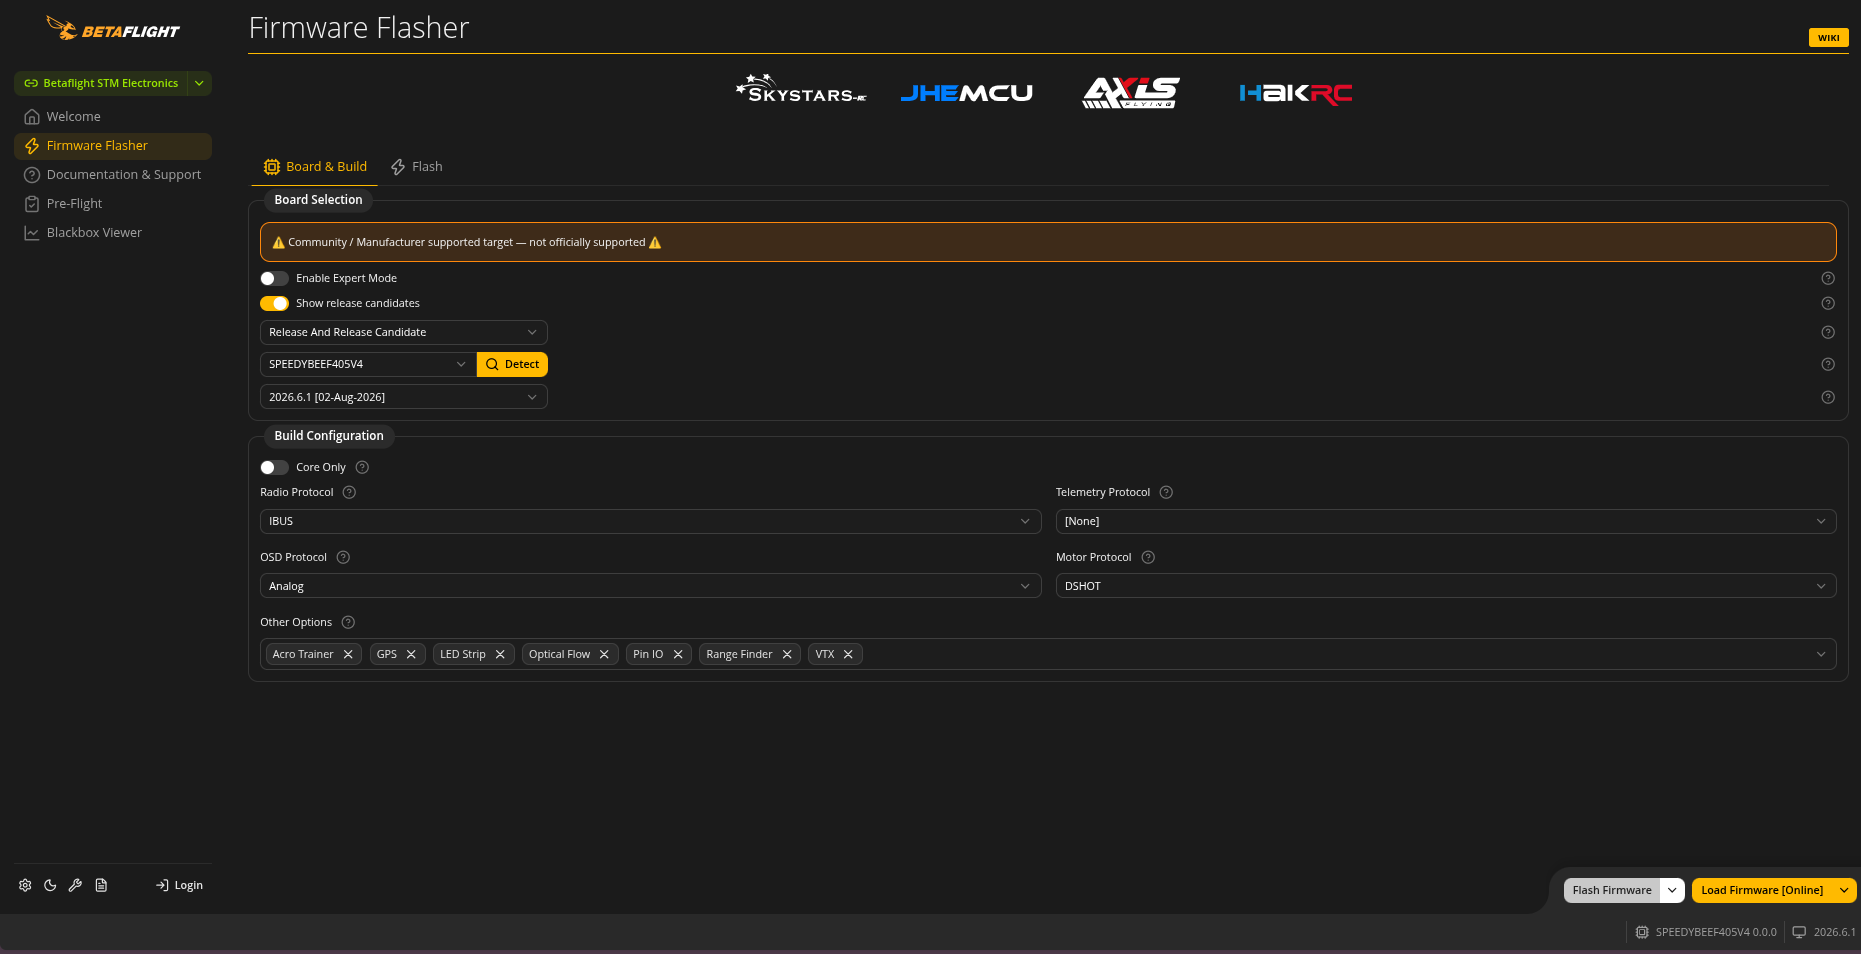
\includegraphics[width=\linewidth]{src//srclog/8-28ConfigFirmware.png}
    \caption{Configuración del firmware en BetaFlight Configurator [Agosto 28, 2026]}
    \label{fig:8-28Config}
\end{figure}
\begin{figure}[!h]
    \centering
    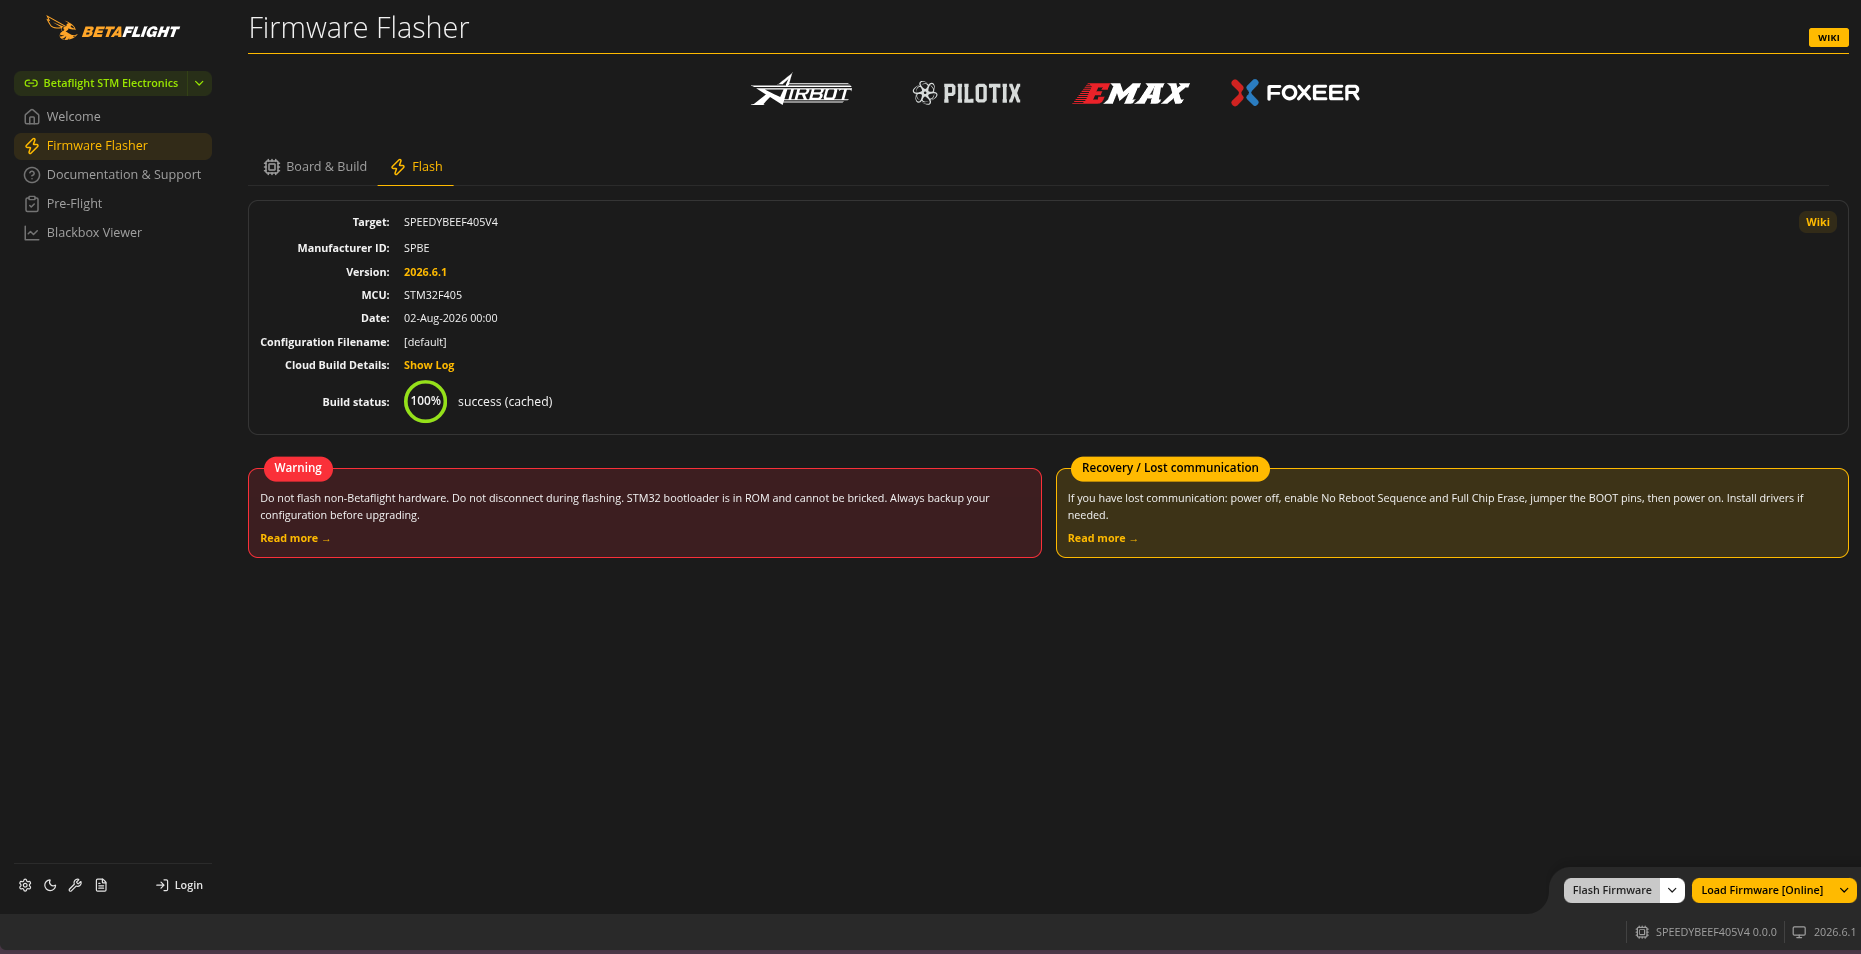
\includegraphics[width=\linewidth]{src//srclog/8-28FirmwareUpdated.png}
    \caption{Firmware BetaFlight 4.4.3 instalado correctamente}
    \label{fig:8-28Updated}
\end{figure}

Se realizó la configuración inicial del sistema:
\begin{itemize}
    \item Receptor configurado en protocolo IBUS sobre el puerto UART2 con mapeo AETR.
    \item Activación del motor/armado asignado al canal auxiliar AUX1.
    \item Protocolo de motores DSHOT300 y configuración de giro inverso (\textit{props out}: \texttt{yaw\_motors\_reversed = ON}).
    \item Ajustes iniciales en el perfil PID 0 (reducción del término D en roll/pitch).
\end{itemize}

\section{Septiembre 2026}
\subsection{7 de Septiembre}
\subsubsection{Aprendizajes}
Se soldaron los componentes de alimentación y señal para integrar la SpeedyBee. Se identificó el receptor modelo \textbf{FS-iA6B}, el cual soporta los protocolos PPM (transmisión canal por canal con mayor cableado) e I-BUS (comunicación serial por un solo hilo). Se optó por utilizar I-BUS para la comunicación con la controladora.

\begin{figure}[!h]
    \centering
    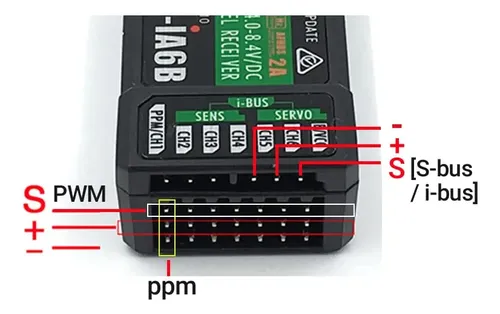
\includegraphics[width=0.5\linewidth]{src/srclog/FS.png}
    \caption{Transmisor FS-iA6B}
    \label{fig:transmisor_fs}
\end{figure}

La soldadura de los pines de alimentación en los pads de gran grosor del ESC presentó dificultad debido a que el disipador interno disipaba rápidamente el calor del cautín. El Dr. Raygoza sugirió el uso de una pistola de calor para facilitar la transferencia térmica en futuras ocasiones.

\subsection{14 de Septiembre \label{sec:9-intentos}}
\subsubsection{Aprendizajes}
Durante septiembre y principios de octubre se realizaron varios intentos de vuelo sin éxito. En los primeros intentos los motores giraban pero el dron no lograba levantar. Para intentar solucionarlo se invirtió el sentido de giro de los motores, con lo que el dron ya levantaba, pero al despegar daba un pequeño brinco y se apagaba.

También se probaron otras configuraciones, como activar el DShot bidireccional con su preset de filtros y cambiar de perfil PID, sin que el dron lograra volar. La causa de estos problemas se identificó y corrigió en la sección \ref{sec:10-13}.

\subsubsection{Incidentes y puntos de mejora}
No hubo daños en el dron, sin embargo se identificaron los siguientes puntos de mejora:
\begin{itemize}
    \item Se realizaron cambios sin entender la causa del problema (por ejemplo, invertir los motores), lo que generó nuevos problemas. Antes de cambiar una configuración se debe diagnosticar primero.
    \item No se contaba con registros del \textit{blackbox}, que hubieran permitido ver por qué se apagaba el dron.
\end{itemize}

\section{Octubre 2026}
\subsection{7 de Octubre}
\subsubsection{Aprendizajes}
Mediante la CLI de BetaFlight vía USB (\texttt{/dev/ttyACM0}) y scripts de diagnóstico en Python, se verificó el estado del hardware:
\begin{itemize}
    \item Sensores íntegros: giroscopio ICM42688P, barómetro DPS310 y OSD MAX7456 detectados sin errores en el bus I2C.
    \item Receptor en UART2 por IBUS verificado y canales mapeados correctamente.
    \item La bandera \texttt{RXLOSS} aparecía correctamente al apagar la emisora.
\end{itemize}

El síntoma reportado era que el dron se armaba, daba un pequeño brinco y se apagaba. Se identificó que este comportamiento corresponde a la protección \textit{Runaway Takeoff Prevention} de BetaFlight, la cual desarma el dron cuando detecta que el lazo PID se satura justo después del despegue. Esta protección se activa cuando el dron no sube derecho, es decir, cuando hay un error en el orden de los motores, en el sentido de giro o en la colocación de las hélices.

Se encontró que los motores habían sido invertidos a propósito, ya que en la configuración correcta el dron no levantaba. La causa real era que las hélices estaban colocadas al revés (empujaban el aire hacia arriba); al invertir los motores el dron sí levantaba, pero el torque de yaw quedaba al contrario de lo que espera BetaFlight, provocando que la corrección de yaw empeorara el giro y se activara la protección. La solución fue intercambiar las hélices y regresar los motores a su sentido correcto para \textit{props out}:

\begin{table}[!h]
\centering
\caption{Sentido de giro para configuración \textit{props out} (vista superior)}
\label{tab:giro}
\begin{tabular}{lll}
\hline
Motor & Posición & Sentido \\
\hline
M1 & Trasero derecho & Antihorario \\
M2 & Delantero derecho & Horario \\
M3 & Trasero izquierdo & Horario \\
M4 & Delantero izquierdo & Antihorario \\
\hline
\end{tabular}
\end{table}
\begin{figure}[!h]
    \centering
    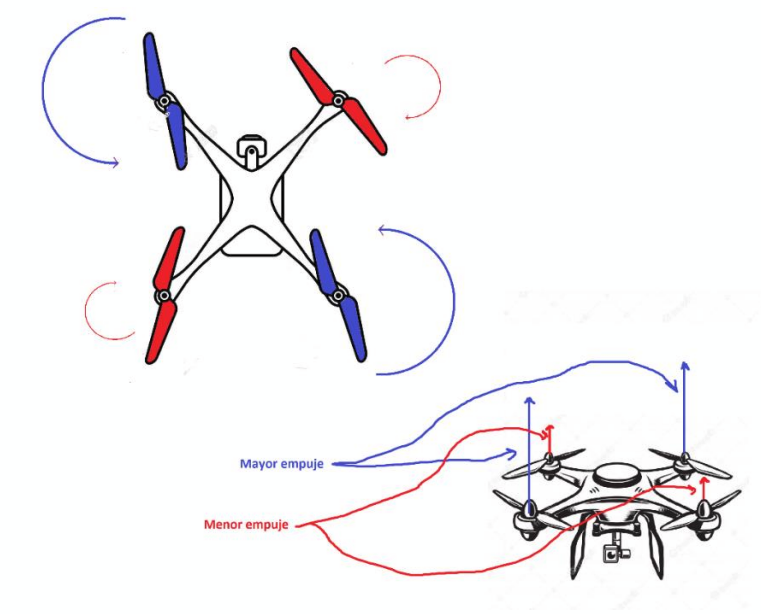
\includegraphics[width=0.6\linewidth]{src/srclog/axis.png}
    \caption{Orden de los motores}
    \label{fig:axis}
\end{figure}
\newpage
\subsection{10 de Octubre \label{sec:10-13}}
\subsubsection{Aprendizajes}
Se probaron configuraciones recomendadas por la comunidad. Al activar el DShot bidireccional (\texttt{dshot\_bidir = ON}) sin contar con telemetría de RPM activa en los ESC, el sistema arrojó un error de filtro RPM (figura \ref{fig:rpm_error}), por lo que se restablecieron los valores predeterminados.

\begin{figure}[!h]
    \centering
    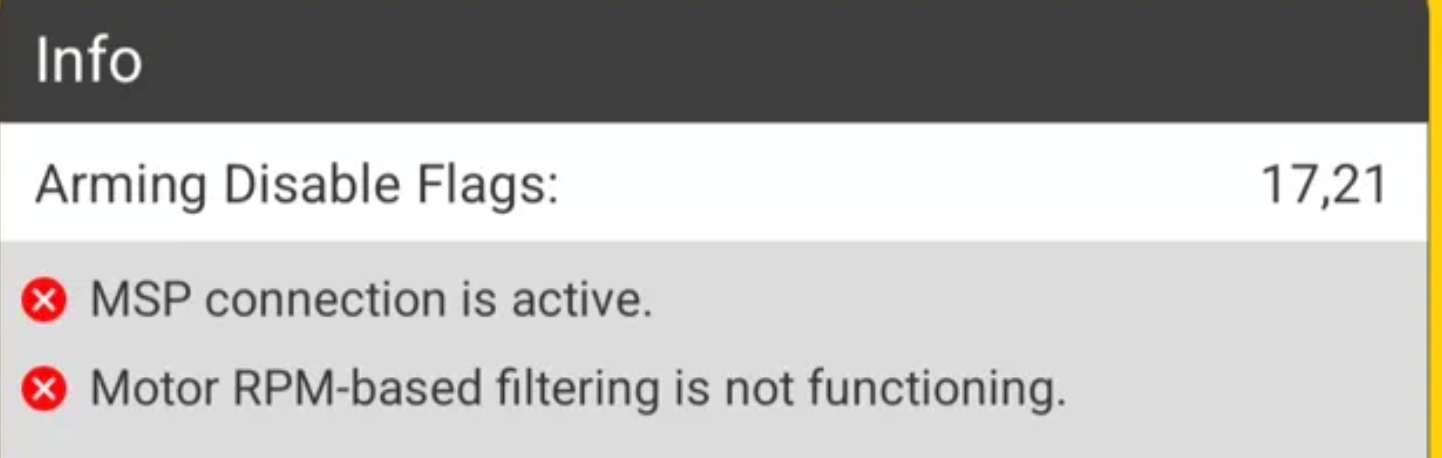
\includegraphics[width=\linewidth]{src/srclog/RPM.png}
    \caption{Alerta de filtro RPM por ausencia de telemetría}
    \label{fig:rpm_error}
\end{figure}

Esta se debía a que se había activado el DShot bidireccional (\texttt{dshot\_bidir = ON}) junto con un preset de filtros que asumen el filtro RPM activo, pero los ESC no estaban enviando telemetría de RPM, entonces se decidió regresar a las configuraciones por default. (Es otro tunning que sale como sugerido)

\subsection{13 de Octubre}
\subsubsection{Aprendizajes}

Una vez con el dron funcionando solo quedaba calibrar el PID de acuerdo a las necesidades. Con el objetivo de que el dron sea más fácil de controlar (vuelo suave, apto para principiantes), se realizaron los cambios mostrados en la tabla \ref{tab:cambios10-13}. Todos los cambios fueron guardados con \texttt{save} y verificados con \texttt{diff} después del reinicio.

\begin{table}[!h]
\centering
\caption{Parámetros ajustados en BetaFlight [Octubre 13, 2026]}
\label{tab:cambios10-13}
\begin{tabular}{lll}
\hline
Parámetro & Antes & Después \\
\hline
\texttt{dshot\_bidir} & ON & OFF \\
Perfil PID / Rates & 2 / 1 & 0 / 0 \\
Filtros del giroscopio & Preset RPM & Default \\
Modo ANGLE & No asignado (Acro) & Siempre activo \\
\texttt{level\_limit} & 55° & 30° \\
Rates roll/pitch (centro/máx/expo) & 70/670/0 & 40/300/0.40 \\
Calibración del acelerómetro & Pendiente & Ajustada en superficie plana \\
\hline
\end{tabular}
\end{table}

Los valores PID quedaron en los valores por defecto de BetaFlight 4.4 (P/I/D/FF de roll 45/80/40/120, pitch 47/84/46/125 y yaw 45/80/0/120), los cuales están pensados para un dron de 5 pulgadas como el LS210. La calibración del acelerómetro se realizó mediante el comando MSP 205 con el dron en una superficie plana.

Con estos cambios se realizó una prueba de vuelo y el dron logró volar de forma estable por primera vez con la nueva controladora, cerrando los problemas descritos en la sección \ref{sec:9-intentos}.

\subsubsection{Incidentes y puntos de mejora}
No hubo incidentes físicos este día, sin embargo se identificaron los siguientes puntos de mejora:
\begin{itemize}
    \item El dron volaba en modo Acro ya que no había ningún modo de vuelo asignado, lo cual dificulta mucho el control; se asignó el modo ANGLE (autonivelado).
\end{itemize}
\begin{figure}[!h]
    \centering
    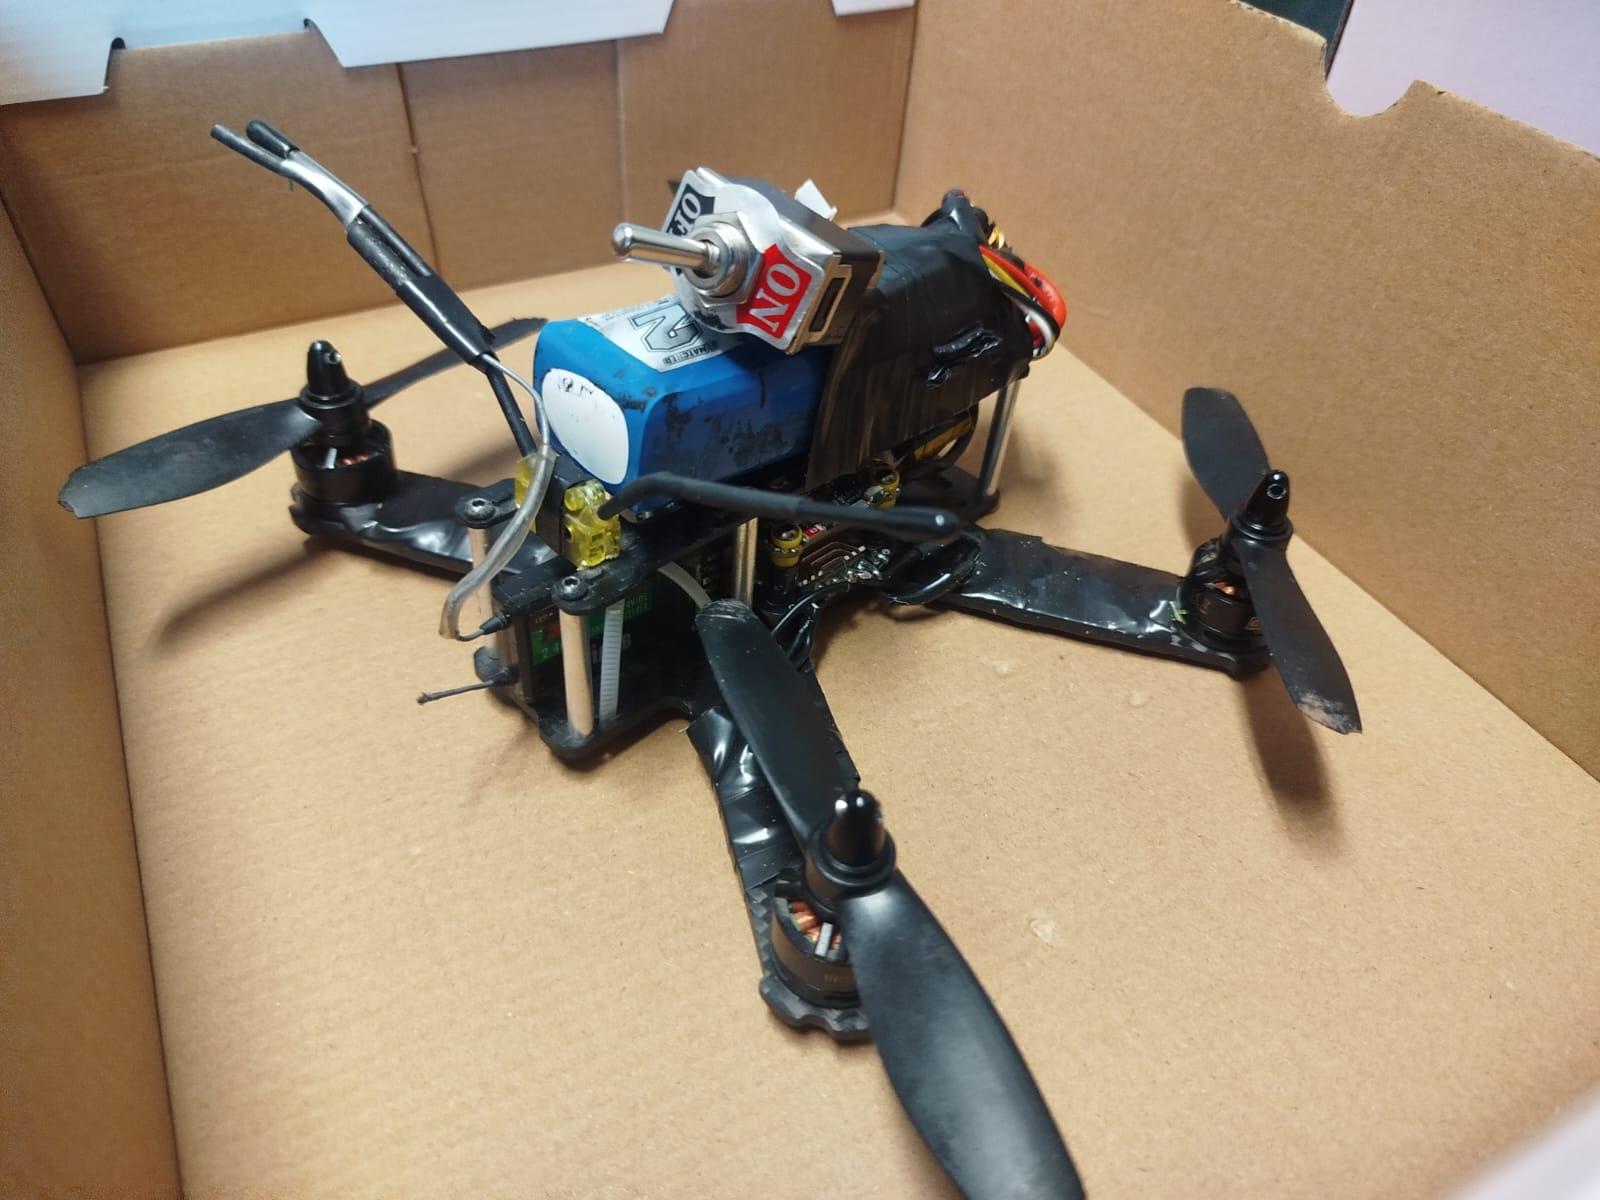
\includegraphics[width=0.5\linewidth]{src/srclog/Dron.png}
    \caption{Dron Funcional}
    \label{fig:DronFuncional}
\end{figure}

Se puede concluir entonces que, El dron..
\begin{itemize}
    \item Ya puede volar de forma estable.
    \item Cuenta con dos interruptores para armar y energizar de forma independiente.
    \item Tiene la capacidad para integrar un diseño mas completo con FPV, GPS o SD. Aprovechándose la potencia que el Speedy Bee ofrece.
\end{itemize}

\subsection{23 de Octubre \label{sec:10-23}}
\subsubsection{Aprendizajes}
El objetivo de este día fue que el dron pudiera mantener su altura de forma automática (\textit{altitude hold}), aprovechando el barómetro DPS310 que ya integra la SpeedyBee F405 V4. BetaFlight 4.4.3 no cuenta con esta función, la cual fue incorporada a partir de la versión 2025.12, por lo que fue necesario actualizar el firmware. El dron no cuenta con GPS ni sensor de flujo óptico, por lo que puede mantener la altura pero no su posición horizontal.

Antes de actualizar se respaldó la configuración completa con el comando \texttt{diff all} desde la terminal. Después se compiló el firmware BetaFlight 2026.6.2 en el servicio en línea de BetaFlight (\textit{cloud build}) con las siguientes opciones:
\begin{itemize}
    \item \textit{Target}: \texttt{SPEEDYBEEF405V4}.
    \item Protocolo de radio: IBUS. Protocolo de OSD: analógico. Protocolo de motores: DSHOT.
    \item Opciones adicionales: \textit{Altitude Hold} y \textit{Position Hold}, además de GPS, \textit{Optical Flow} y \textit{Range Finder} para futuras ampliaciones.
\end{itemize}

La instalación presentó varios problemas:
\begin{itemize}
    \item En el navegador Brave el configurador no lograba acceder al dispositivo, y Firefox no permite flashear porque no soporta WebUSB, el cual es necesario para comunicarse con la controladora en modo DFU (\textit{Device Firmware Upgrade}).
    \item La orden del configurador para reiniciar la controladora en modo DFU no funcionaba: la placa se reiniciaba en modo normal y el configurador se quedaba esperando.
\end{itemize}

La solución fue realizar el proceso desde la terminal. Primero se envió el comando \texttt{bl} por la CLI, con el cual la controladora se reinició en modo DFU (identificador USB \texttt{0483:df11}, \textit{STM32 BOOTLOADER}). Después se descargó el archivo \texttt{.hex} desde el configurador y se grabó con la herramienta \texttt{dfu-util}, realizando un borrado completo de la memoria (\textit{mass erase}). El archivo contiene dos bloques de memoria (vectores en \texttt{0x08000000} y firmware a partir de \texttt{0x08008000}), por lo que se grabaron por separado para no escribir sobre el área de configuración. La controladora arrancó correctamente con BetaFlight 2026.6.2, detectando todos sus sensores.

Al haber borrado la memoria, se volvió a aplicar la configuración por la terminal (tabla \ref{tab:cambios10-23}). En esta versión algunos parámetros cambiaron de nombre, por ejemplo \texttt{level\_limit} ahora es \texttt{angle\_limit}. El modo ALTHOLD se asignó al canal AUX2 (canal 6 del receptor), el cual se activó en el transmisor y se verificó en el configurador.

\begin{table}[!h]
\centering
\caption{Configuración aplicada en BetaFlight 2026.6.2 [Octubre 23, 2026]}
\label{tab:cambios10-23}
\begin{tabular}{ll}
\hline
Parámetro & Valor \\
\hline
Receptor & IBUS en UART2, mapeo AETR \\
\texttt{motor\_pwm\_protocol} & DSHOT300 \\
\texttt{yaw\_motors\_reversed} & ON (\textit{props out}) \\
Armado & AUX1, 1950--2075 \\
Modo ANGLE & Siempre activo \\
Modo ALTHOLD (nuevo) & AUX2, 1700--2100 \\
\texttt{angle\_limit} & 30° \\
Rates & Mismos del 13 de octubre \\
Calibración del acelerómetro & Restaurada del respaldo \\
\texttt{small\_angle} & 25° (valor por defecto) \\
PID y filtros & Valores por defecto de 2026.6.2 \\
\hline
\end{tabular}
\end{table}

\subsubsection{Incidentes y puntos de mejora}
\begin{itemize}
    \item En los vuelos anteriores se observó que, en modo ANGLE, el dron no respondía al movimiento lateral (\textit{roll}) hacia ningún lado, mientras que adelante y atrás (\textit{pitch}) sí respondía. Se verificó en el configurador que el canal de roll llega completo (de 1000 a 2000), por lo que el problema no está en el control. Queda pendiente revisar el orden físico de los motores y los valores que la controladora envía a cada motor.
    \item El peso del dron es de 497\,g, mientras que el empuje de los cuatro motores BE1806 según el fabricante es de alrededor de 520\,g. La relación empuje/peso es muy cercana a 1:1, lo que deja poco margen para maniobrar y para que el modo ALTHOLD corrija la altura.
    \item Se debe colocar espuma sobre el barómetro para que el flujo de aire de las hélices no altere la medición de presión.
    \item Queda pendiente la prueba de vuelo de ALTHOLD y ajustar el parámetro \texttt{ap\_hover\_throttle} con el valor real del acelerador necesario para flotar.
    \item Los respaldos de la configuración se guardaron en la carpeta \texttt{respaldos} del proyecto.
\end{itemize}
\newpage
\section{Anexos}

\appendix
\renewcommand{\thesubsection}{\Roman{subsection}}

\subsection{Tabla de componentes y refacciones \label{sec:TablaComponentes}}
\begin{table}[!h]
\centering
\caption{Componentes adquiridos, fabricados y recibidos}
\label{tab:componentes}
\begin{tabular}{p{4.6cm}p{2.2cm}p{2.2cm}p{1.8cm}}
\hline
Componente & Estado & Proveedor  & Fecha \\
\hline
\textit{Stack} SpeedyBee F405 V4 BLS 55A (FC + ESC 4 en 1) & Instalado & AliExpress  & Junio 2026 \\
Interruptor de 1 polo y 2 posiciones (energizado) & Instalado   & AliExpress & Abril 2026 \\
Base de pruebas para ajuste de PID (base de ventilador adaptada) & Fabricada & Fabricación propia  & Junio 2026 \\
Cables soldados al puerto SWD & Fabricado & Fabricación propia  & Mayo 2026 \\
Receptor FS-iA6B (protocolo I-BUS) & Reutilizado & Incluido con el dron  & Sep 2026 \\
Controladora CC3D EVO & Retirada (dañada) & Incluida con el dron  & Marzo 2026 \\
\hline
\end{tabular}
\end{table}
\newpage
\subsection{LibrePilot}
\subsubsection{Actualización de Firmware \label{sec:Firmware}}
Para actualizar el firmware en LibrePilot se deben seguir los siguientes pasos:
\begin{enumerate}
    \item Abrir el software LibrePilot y conectar el dron mediante el cable USB.
    \item Ir a la sección de configuración del firmware haciendo clic en el icono superior derecho (figura \ref{fig:Firmware}).
    \item Verificar la correcta detección del puerto.
    \item Desconectar el cable USB.
    \item Seleccionar la opción \textit{Upgrade \& Erase}.
    \item Conectar inmediatamente el cable USB para permitir que el cargador de arranque (\textit{bootloader}) reciba el paquete de actualización.
\end{enumerate}

\begin{figure}[!h]
    \centering
    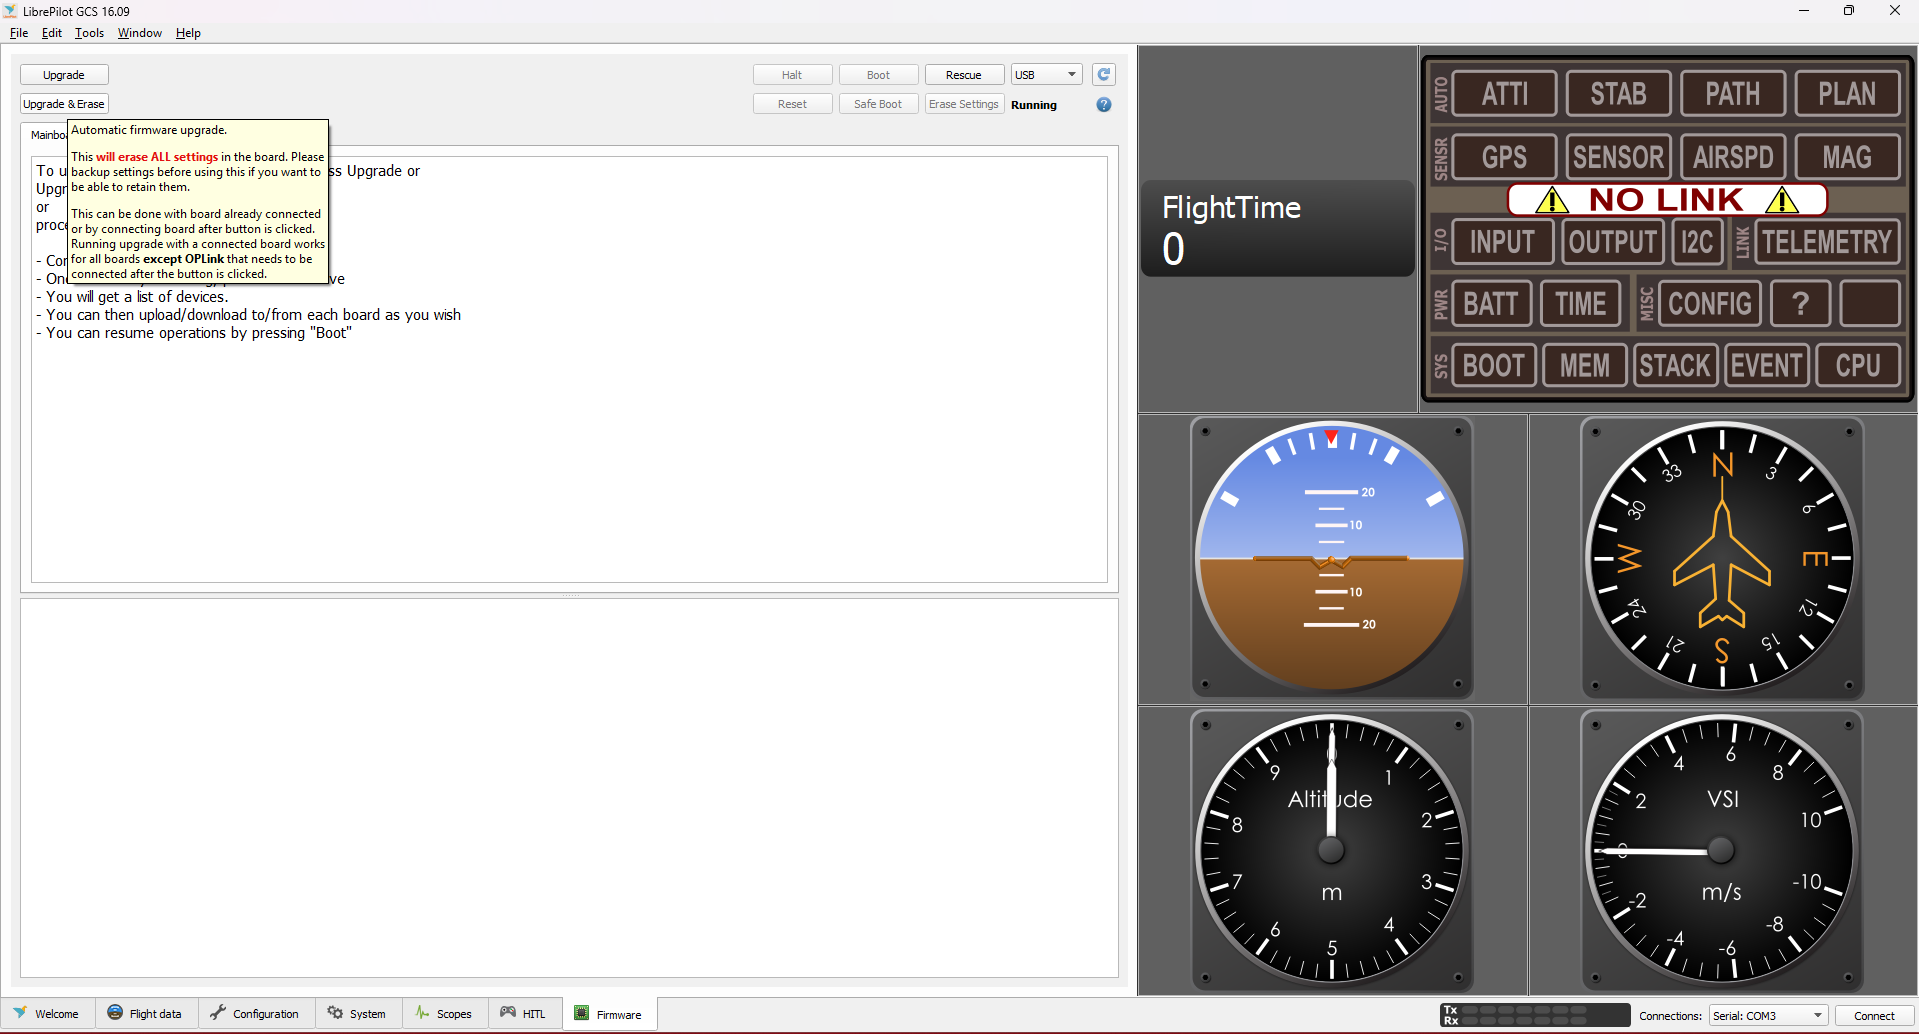
\includegraphics[width=0.8\linewidth]{src//srclog/FirmwareUpdate.png}
    \caption{Pestaña de configuración de firmware en LibrePilot}
    \label{fig:Firmware}
\end{figure}

\begin{figure}[!h]
    \centering
    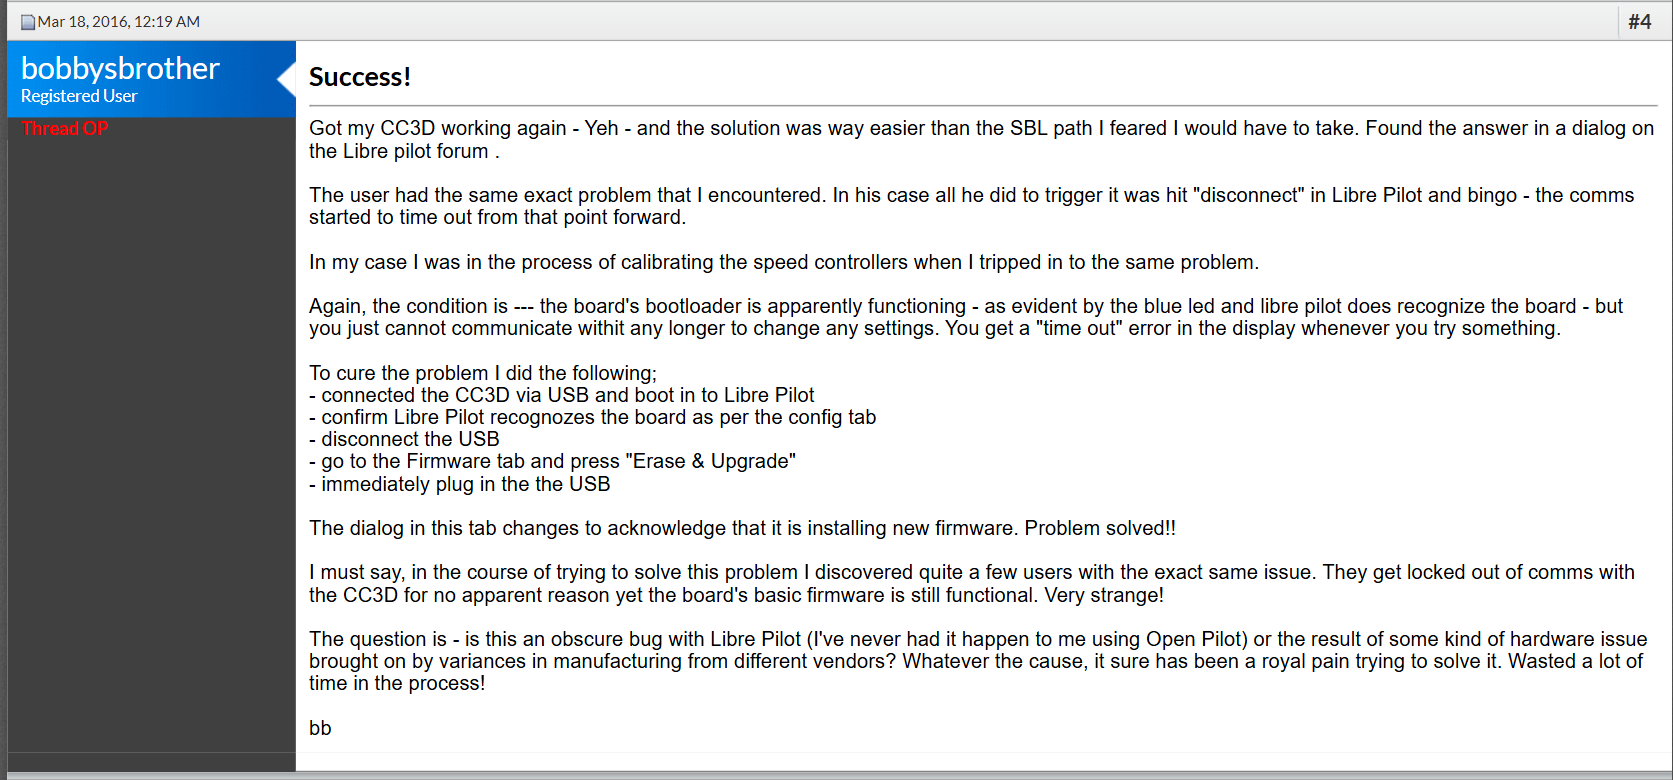
\includegraphics[width=\linewidth]{src//srclog/FirmwareUpdateforo.png}
    \caption{Referencia del foro sobre el procedimiento de actualización}
    \label{fig:Firmwareforo}
\end{figure}

\newpage

%% ============================== 6 ==============================
\section{Manual de operación}
\label{sec:manual}
Esta sección describe cómo utilizar el dron desde la preparación de la batería hasta el apagado. Se recomienda leerla completa antes del primer vuelo junto con los procedimientos de seguridad (sección \ref{sec:seguridad}).

\subsection{Controles del transmisor}
El transmisor se utiliza en modo 2. La tabla \ref{tab:controles} indica la función de cada control.

\begin{table}[!h]
\centering
\caption{Controles del transmisor (modo 2)}
\label{tab:controles}
\begin{tabularx}{\textwidth}{@{}llX@{}}
\toprule
\textbf{Control} & \textbf{Canal} & \textbf{Función} \\
\midrule
Stick izquierdo, arriba/abajo & Throttle & Acelerador: sube o baja el dron \\
Stick izquierdo, izquierda/derecha & Yaw & Gira el dron sobre su propio eje \\
Stick derecho, arriba/abajo & Pitch & Inclina el dron hacia adelante o hacia atrás \\
Stick derecho, izquierda/derecha & Roll & Inclina el dron hacia los lados \\
Interruptor del canal 5 & AUX1 & Armado: arriba arma los motores, abajo los desarma \\
Interruptor del canal 6 & AUX2 & ALTHOLD: arriba mantiene la altura, abajo vuelo normal \\
\bottomrule
\end{tabularx}
\end{table}

Los interruptores de los canales 5 y 6 se asignan en el menú \textit{Functions setup} $\rightarrow$ \textit{Aux. channels} del transmisor FlySky. Ambos deben estar abajo antes de encender el dron.

\begin{figure}[!h]
    \centering
    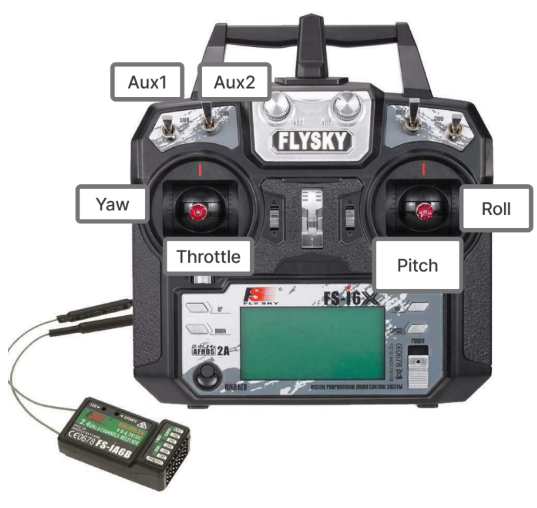
\includegraphics[width=0.5\linewidth]{src/srclog/Control FS-ia6b.png}
    \caption{Control Flysky}
    \label{fig:placeholder}
\end{figure}

\subsection{Batería}
La batería es una LiPo de 3 celdas (3S). Cada celda tiene un voltaje nominal de 3.7\,V; la tabla \ref{tab:bateria} muestra los voltajes de referencia.

\begin{table}[!h]
\centering
\caption{Voltajes de referencia de la batería LiPo 3S}
\label{tab:bateria}
\begin{tabular}{@{}lcc@{}}
\toprule
\textbf{Estado} & \textbf{Por celda} & \textbf{Total (3S)} \\
\midrule
Carga completa & 4.20\,V & 12.6\,V \\
Almacenamiento (si no se usará en días) & 3.80\,V & 11.4\,V \\
Alerta de BetaFlight: aterrizar & 3.50\,V & 10.5\,V \\
Mínimo absoluto, no descargar por debajo & 3.30\,V & 9.9\,V \\
\bottomrule
\end{tabular}
\end{table}

\begin{itemize}[nosep]
    \item Cargar siempre con un cargador balanceador y bajo supervisión.
    \item Antes de volar, revisar el voltaje de cada celda con el checador \logref{Marzo 13}. Las tres celdas deben tener voltajes similares (diferencia menor a 0.1\,V).
    \item No utilizar una batería inflada o golpeada.
\end{itemize}

\subsection{Encendido}
\begin{enumerate}[nosep]
    \item Encender primero el transmisor, con el acelerador al mínimo y los interruptores AUX1 y AUX2 abajo.
    \item Colocar el dron en una superficie plana, lejos de personas.
    \item Conectar la batería o activar el interruptor de energía sujetando el dron contra el suelo \logref{Marzo 13}.
    \item Esperar los tonos de inicio de los ESC y no mover el dron durante unos segundos, ya que la controladora calibra el giroscopio al encender.
\end{enumerate}

\subsection{Armado y despegue}
\begin{enumerate}[nosep]
    \item Con el acelerador al mínimo, subir el interruptor AUX1 para armar.
    \item \textbf{Importante:} con la función \texttt{MOTOR\_STOP}, los motores no giran aunque el dron esté armado si el acelerador está en cero. \textbf{Un dron armado debe tratarse siempre como si los motores estuvieran girando.}
    \item Subir el acelerador de forma suave hasta que el dron despegue y estabilizarlo a una altura de 1 a 2\,m.
\end{enumerate}
Si el dron no arma, revisar las banderas de armado (sección \ref{sec:problemas}). Las causas más comunes son que el acelerador no está al mínimo, que el dron está inclinado más de 25$^{\circ}$ o que no hay señal del transmisor.

\subsection{Vuelo en modo ANGLE}
El modo ANGLE está siempre activo. En este modo el stick derecho controla el ángulo de inclinación del dron (máximo 30$^{\circ}$) y, al soltarlo, el dron regresa a la posición nivelada. El acelerador controla la altura y el stick izquierdo horizontal gira el dron. Se recomienda realizar movimientos pequeños y suaves, y mantener el dron siempre a la vista.

\subsection{Mantenimiento de altura (ALTHOLD)}
\begin{enumerate}[nosep]
    \item Despegar y estabilizar el dron a una altura de 1 a 2\,m en vuelo normal.
    \item Subir el interruptor AUX2. El dron mantendrá la altura en la que se encontraba.
    \item Colocar el acelerador en el centro. Moverlo hacia arriba o abajo hace que el dron suba o baje de forma controlada, y al regresarlo al centro mantiene la nueva altura.
    \item El dron no mantiene su posición horizontal: el viento lo desplaza, por lo que se debe corregir con el stick derecho.
    \item Si el dron sube, baja u oscila de forma brusca, bajar el interruptor AUX2 de inmediato y retomar el control con el acelerador.
\end{enumerate}

\subsection{Aterrizaje y apagado}
\begin{enumerate}[nosep]
    \item Si ALTHOLD está activo, bajar el interruptor AUX2.
    \item Bajar el acelerador suavemente hasta que el dron toque el suelo.
    \item Llevar el acelerador al mínimo y bajar el interruptor AUX1 para desarmar.
    \item Desconectar la batería o apagar el interruptor de energía. Apagar el transmisor siempre al final.
\end{enumerate}

\subsection{Emergencias}
\begin{itemize}[nosep]
    \item \textbf{Pérdida de control:} bajar el interruptor AUX1. Los motores se detienen de inmediato y el dron cae, por lo que se debe hacer cuando el dron está a baja altura o en una zona despejada.
    \item \textbf{Pérdida de señal:} si el dron deja de recibir la señal del transmisor por 1.5\,s, apaga los motores y cae (\textit{failsafe} en modo DROP). Por ello se debe volar siempre dentro del alcance del transmisor.
    \item \textbf{Brinco al despegar y desarmado:} es la protección \textit{Runaway Takeoff}. No se debe volver a intentar el vuelo hasta revisar las hélices y el sentido de giro de los motores.
\end{itemize}

\subsection{Después del vuelo}
\begin{itemize}[nosep]
    \item Revisar la temperatura de los motores con la mano: deben estar tibios, no calientes.
    \item Revisar que las hélices no estén dañadas y sigan apretadas.
    \item Medir el voltaje de la batería y dejarla en voltaje de almacenamiento si no se volverá a usar en los siguientes días.
\end{itemize}

\subsection{Conexión a la computadora}
\begin{itemize}[nosep]
    \item \textbf{BetaFlight Configurator:} se utiliza desde \url{https://app.betaflight.com} en Chrome o Chromium. Firefox no permite actualizar el firmware y Brave bloquea el acceso al USB por defecto.
    \item \textbf{Aplicación SpeedyBee:} permite configurar el dron por Bluetooth desde el teléfono.
    \item \textbf{Terminal:} con los scripts de Python del anexo \ref{anx:cli} se pueden consultar y modificar los parámetros directamente.
    \item Antes de probar motores desde la computadora se deben retirar las hélices. Para probar los motores o el receptor es necesario conectar la batería, ya que el USB no alimenta al ESC.
\end{itemize}

%% ============================== 7 ==============================
\section{Guía de solución de problemas}
\label{sec:problemas}
La tabla \ref{tab:problemas} reúne los problemas encontrados durante el proyecto, su causa y su solución. Las banderas (\textit{flags}) se consultan con el comando \texttt{status} en la línea \textit{Arming disable flags}, o en la pestaña \textit{Setup} del BetaFlight Configurator.

\begin{table}[!h]
\centering
\caption{Problemas frecuentes y su solución}
\label{tab:problemas}
\small
\begin{tabularx}{\textwidth}{@{}>{\raggedright\arraybackslash}p{3.2cm}>{\raggedright\arraybackslash}X>{\raggedright\arraybackslash}X>{\raggedright\arraybackslash}p{2.1cm}@{}}
\toprule
\textbf{Síntoma} & \textbf{Causa} & \textbf{Solución} & \textbf{Log File} \\
\midrule
Los motores giran pero el dron no levanta &
Hélices colocadas al revés: empujan el aire hacia arriba &
Colocar en cada motor la hélice de su sentido de giro (borde de ataque primero) &
Sept., 7 Oct. \\
\addlinespace
Despega con un brinco y se desarma &
Protección \textit{Runaway Takeoff}: el giro de los motores no coincide con \texttt{yaw\_motors\_reversed}, o hay motores fuera de orden &
Verificar orden y giro (tabla \ref{tab:motores}). No invertir motores sin invertir también las hélices &
Sept., 7 Oct. \\
\addlinespace
Bandera \texttt{RXLOSS} &
No llega señal del receptor &
Encender el control, verificar el enlace y la alimentación del receptor &
7 Oct. \\
\addlinespace
Bandera \texttt{RPMFILTER} &
DShot bidireccional activo sin telemetría de los ESC &
Conectar la batería; si persiste, \texttt{set dshot\_bidir = OFF} &
10 Oct. \\
\addlinespace
Bandera \texttt{NO\_ACC\_CAL} &
Modo ANGLE activo con acelerómetro sin calibrar &
Calibrar el acelerómetro en superficie plana (pestaña \textit{Setup}) &
13 Oct. \\
\addlinespace
Banderas \texttt{CLI}, \texttt{MSP} o \texttt{CALIB} &
Conexión a la PC o calibración del giroscopio en curso &
Desconectar el USB; mantener el dron quieto al energizar &
13 Oct. \\
\addlinespace
El dron se carga hacia un lado &
Acelerómetro sin calibrar o desbalance físico &
Calibrar el acelerómetro; revisar hélices y centro de masa &
Marzo 27 \\
\addlinespace
No responde al movimiento lateral (roll) &
En diagnóstico: posible error en el orden físico de los motores o falta de empuje (relación empuje/peso cercana a 1:1) &
Verificar en la pestaña \textit{Motors} que cada motor corresponda a su posición (tabla \ref{tab:motores}) &
23 Oct. \\
\addlinespace
ALTHOLD sube, baja u oscila &
Acelerador de \textit{hover} mal estimado o flujo de aire sobre el barómetro &
Ajustar \texttt{ap\_hover\_throttle}; cubrir el barómetro con espuma &
23 Oct. \\
\addlinespace
El configurador no actualiza el firmware o no entra en DFU &
El navegador no soporta WebUSB (Firefox) o lo bloquea (Brave) &
Usar Chrome o Chromium, o grabar desde la terminal con \texttt{bl} y \texttt{dfu-util} (anexo \ref{anx:flash}) &
23 Oct. \\
\addlinespace
\texttt{SD card: Startup failed} &
No hay tarjeta microSD o no tiene formato válido &
Insertar microSD en formato FAT32 para el \textit{blackbox} &
13 Oct. \\
\bottomrule
\end{tabularx}
\end{table}

%% ============================== 8 ==============================
\section{Procedimientos de seguridad}
\label{sec:seguridad}
Las siguientes reglas se derivan de los incidentes registrados en el \textit{Log File}:

\noindent\textbf{Antes de volar}
\begin{enumerate}[nosep]
    \item Revisar el voltaje de cada celda de la batería con un checador, conectando negativo con negativo \logref{Marzo 13}.
    \item Verificar que las tuercas de las hélices estén apretadas \logref{Marzo 13}.
    \item Sujetar la batería y su cable lejos de las hélices \logref{Marzo 13, 1 de Abril}.
    \item Colocar los controles del radio en su posición por defecto, el acelerador en cero y los interruptores AUX1 y AUX2 abajo \logref{Marzo 13}.
    \item Volar únicamente en el estadio, lejos de salones y automóviles, sin exceder la altura permitida \logref{Marzo 27}.
\end{enumerate}

\noindent\textbf{Durante la configuración}
\begin{enumerate}[nosep]
    \item Retirar las hélices antes de probar motores desde la PC.
    \item Configurar siempre con el dron desarmado \logref{Marzo 27}.
    \item Guardar un respaldo con \texttt{diff all} antes de realizar cambios \logref{23 de Octubre}.
    \item No desactivar la protección \textit{Runaway Takeoff}.
\end{enumerate}

\begin{thebibliography}{99}

\bibitem{FirmwareUpdate}
Bobby's Brother (Marzo 18, 2016). \textit{CC3D bootloader problem}. Recuperado de \url{https://www.rcgroups.com/forums/showthread.php?2626688-CC3D-bootloader-problem}

\bibitem{TorrenteDigital}
Torrente Digital (2017). \textit{Eachine Racer 250 con FlySky FS-iA6 Configuración LibrePilot}. Recuperado de \url{https://youtu.be/1uklcI0D6_w?si=e9yl_73H5cXIJYUo}

\bibitem{stm32ventajas}
Ampheo (2025). \textit{Which microcontrollers are used in drones?}. Recuperado de \url{https://www.ampheo.com/blog/which-microcontrollers-are-used-in-drones}

\bibitem{rogerlipo}
Brian Schneider (2021). \textit{A Guide to Understanding LiPo Batteries}. Recuperado de \url{https://www.rogershobbycenter.com/lipoguide}

\bibitem{gensacelipo}
Tattu Gens Ace (2024). \textit{LiPo Battery Guide}. Recuperado de \url{https://gensace.de/pages/lipo-battery-guide}

\bibitem{rclipo}
Guides d'achat (2025). \textit{The LiPo Battery Guide}. Recuperado de \url{https://www.rcteam.com/en/blogs/the-rc-model-blog/lipo-battery-guide}

\end{thebibliography}

\end{document}
